%                                                                 aa.dem
% AA vers. 9.1, LaTeX class for Astronomy & Astrophysics
% demonstration file
%                                                       (c) EDP Sciences
%-----------------------------------------------------------------------
%
% \documentclass[referee]{aa} % for a referee version
%\documentclass[onecolumn]{aa} % for a paper on 1 column  
%\documentclass[longauth]{aa} % for the long lists of affiliations 
% \documentclass[letter]{aa} % for the letters 
%\documentclass[bibyear]{aa} % if the references are not structured 
%                              according to the author-year natbib style

%
\documentclass{aa}  

%
\usepackage{amsmath}
\usepackage{graphicx, comment}
\usepackage{commath}
\usepackage{txfonts}
\usepackage{subfig}
\usepackage{upgreek}
\usepackage{threeparttable} 
\usepackage{booktabs}
\usepackage{siunitx}
\usepackage{natbib}
\usepackage{float}
\usepackage{enumitem}

% \usepackage[backend=biber, style=authoryear, natbib=true]{biblatex}
% 超链接配置：确保链接颜色可见，去除边框
\usepackage[colorlinks=true, linkcolor=blue, urlcolor=blue, citecolor=blue]{hyperref}
\usepackage{orcidlink}

\newcommand{\C}{3C\,84}
\newcommand{\rotang}{-4.5^\circ}
\newcommand{\protang}{4.5^\circ}
\newcommand{\beam}{(0.17\times0.40)\,\textrm{mas}}

\newcommand{\Mj}{5.0\pm1.7}
\newcommand{\Mjrel}{6.7\pm2.0}
\newcommand{\Mx}{9.8\pm3.2}
\newcommand{\enthalpy}{0.26\pm0.20}
\newcommand{\ajj}{0.14\pm0.06}
\newcommand{\ax}{0.07\pm0.02}
\newcommand{\bw}{0.27\pm0.04}

\newcommand{\rj}{0.36\pm0.09\,\textrm{pc}}
\newcommand{\phij}{4.5^\circ\pm1.2^\circ}
\newcommand{\thetaj}{35^\circ\pm5^\circ}
\newcommand{\gj}{1.35\pm0.14}


\newcommand{\tp}{30\pm10\,\textrm{years}}
\newcommand{\chiamp}{\sim1}
\newcommand{\chialt}{\sim2}




\begin{document} 

\renewcommand{\arraystretch}{1.5}
   
    \title{
    % 1.4GHz下对低红移射电星系的统计：用多种视角观察射电星系的特性
    Morphology Statistics of the Fanaroff-Riley I and II Sources
    }

    \author{
        P.-G. Zheng\inst{1,2}
    \and R.-Y. Ma\inst{1,2}\thanks{Corresponding author: \email{ryma@xmu.edu.cn}}
    \and Z.-H. Zhu\inst{3,2}\thanks{Corresponding author: \email{}}
    \and X. Cao\inst{1,2}
    \and Y. Xie\inst{4}\thanks{Corresponding author: \email{xieyi@jmu.edu.cn}}
    \and X.-L. Wang\inst{1,2}
    }
    
    \institute{
    Department of Astronomy and Institute of Theoretical Physics and Astrophysics, Xiamen University, Xiamen, Fujian 361005, China
    \and
    SHAO--XMU Joint Center for Astrophysics, Xiamen, Fujian 361005, China
    \and
    Shanghai Astronomical Observatory, Chinese Academy of Sciences, 80 Nandan Road, Shanghai 200030, China
    \and
    School of Science, Jimei University, Xiamen 361021, Fujian Province, China
    }




   \date{Received -; accepted -}


 \abstract
   {
   Jet lobes of Radio Galaxies (RGs) are vital components shaped primarily by interactions with the circumgalactic medium. This study focuses on extracting morphological parameters of Fanaroff-Riley (FR)\textemdash classified RGs (FRI and FRII) from 1.4 GHz radio images via elliptical structure fitting, aiming to systematically characterize their morphological properties. A semi-automated workflow is developed to localize the RG cores and lobes. 
    Our key results are as follows:
    (1) We performed a systematic statistical analysis of RG morphological properties, adopting the aspect ratio as the primary metric to quantify their structural signatures. Using this framework, we statistically verified the intrinsic physical differences between FRI and FRII populations, and suggest a correlation between the double-lobe brightness ratio and the positional offset ratio of their optical counterparts within the aspect ratio range of [0.2, 0.3].
    (2) We applied the classical $r_s$ method to our full sample, and uncovered a prominent, parameter-insensitive substructure in FRIIs at $r_s$<0.3. This feature is robust against variations in algorithm tuning, which remains stable across different algorithm tuning configurations.
    (2) Via the classical $r_s$ method for sample analysis, and detect a distinct, parameter-insensitive substructure for FRIIs at $r_s$<0.3, which remains stable across different algorithm tuning configurations.
    (3) We perform knot enumeration using a flood-filling approach with a maximum brightness threshold to track the evolutionary characteristics of knot structures, with cross-validation confirming that these knots are not induced by random flux fluctuations.
    (4) We construct the central line of RGs and reveal the average radiatively active regions of RGs via brightness stacking of central lines from a sufficiently large sample.
    Collectively, our multi-perspective analysis clarifies the structural properties and evolutionary mechanisms of FR-classified RGs, and refines the existing understanding of FR morphological classification. In this study, we combine well-established methodologies from prior literature with our novel technical approaches to conduct a comprehensive characterization of FRIs and FRIIs from the Faint Images of the Radio Sky at Twenty-Centimeters (FIRST) survey.
    
   }
 
  

   \keywords{
            Active galactic nuclei; Radio galaxy; Radio astronomy
               }

   \maketitle

   
\section{Introduction}\label{sec:Introduction}
% 介绍RGs重要性
Radio galaxies (RGs) are a class of active galaxies whose prominent radio emission is powered by relativistic jets launched from the central supermassive black hole. Their radio structures span an enormous range of spatial scales, from parsecs to megaparsecs \citep{hardcastle_radio_2020}. It is now well established that luminous RGs play key roles in regulating galaxy evolution and the formation of cosmic large-scale structures \citep{miley_distant_2008}. The general picture of RGs has been widely accepted: the central black hole powers the jet with rotational energy extracted either from the black hole itself via the Blandford–Znajek process or from the accretion flow via the Blandford–Payne process \citep{BZ77,BP82}; the energy is then transferred outward along large-scale magnetic fields, accompanied by the acceleration of bulk motion and relativistic particles. At the jet–ambient medium interface, the external intergalactic medium plays a crucial role in shaping the morphology of the extended radio structure \citep[e.g.,][and references therein]{BlandfordRees1978,ghisellini_bulk_1989,blandford_relativistic_2019}.

Observationally, RGs have been classified in multiple complementary ways according to their morphology, spectral index, emission-line properties, and radio-to-optical flux ratio \citep[e.g.,][]{fanaroff_morphology_1974,osterbrock_broad_1975,heckman_optical_1980,veilleux_spectral_1987,owen_ccd_1989,kellermann_radio_1989}. Among these, the most widely adopted and historically earliest morphological classification is the Fanaroff–Riley (FR) scheme, proposed by \citet{fanaroff_morphology_1974}. This scheme divides extended radio sources into two types based on the ratio 
of the separation between the brightest regions on the two lobes to the total linear size of the radio structure. FRI sources are centre-brightened, with surface brightness decreasing from the core outward along symmetric large-scale jets, and are typically less luminous. FRII sources are edge-brightened, with bright hot spots near the outer extremities of more collimated, often asymmetric jets, and are typically more luminous \citep{ledlow_20cm_1996}.

Subsequent studies have demonstrated that radio luminosity alone is not a reliable indicator for determining FR type: sources with identical radio luminosity can display either FRI or FRII morphology \citep[e.g.,][]{mingo_revisiting_2019}. \citet{ledlow_20cm_1996} found that the FRI/FRII dividing line in the radio-luminosity–optical-magnitude plane is not sharp but rather a function of the host galaxy's optical luminosity, with brighter host galaxies requiring higher radio luminosities for the FRI-to-FRII transition. \cite{lin_populations_2010} further proposed using the ratio as a quantitative diagnostic parameter to discriminate between RGs of different morphologies. A particularly intriguing subset is the hybrid morphology radio sources (HYMORS), first identified by \citet{gopal-krishna_extragalactic_2000}, in which one lobe exhibits FRI structure while the opposite lobe shows FRII structure — a phenomenon that provides strong constraints on theoretical models for the FR dichotomy. 

The physical origin of the FRI/FRII dichotomy has attracted intense theoretical interest. Explanations generally fall into three categories: those invoking intrinsic differences in the central engine \citep[e.g.,][]{Baum1995,Meier1999,hardcastle_radio_2020}, such as black hole spin, accretion mode, or jet composition; those attributing the dichotomy to the external environment, including the location where the initially supersonic jet decelerates or encounters a density jump in the ambient medium \citep[e.g.,][]{de_young_relation_1993,bicknell_relativistic_1995,bowman_deceleration_1996,liu_environment_2019}; and those focusing on the jet itself, such as its initial power and stability \citep[e.g.,][]{florido_spatial_1990,Reynolds1996,Meier1997,lane_3c_2002}. The existence of HYMORS argues strongly against explanations that rely solely on central-engine properties — a single black hole is unlikely to produce jets of fundamentally different natures in opposite directions simultaneously \citep{gopal-krishna_extragalactic_2000} — and instead favors models in which the FR morphology is primarily determined by the jet–environment interaction. This conclusion is further supported by recent relativistic magneto-hydrodynamic simulations, which demonstrate that the plasma properties of the jet --- specifically, the composition (electron--positron versus electron--proton) and the magnetization --- critically determine whether the resulting large-scale morphology resembles an FRI or FRII source \citep{tripathi_how_2026}.
Despite these ongoing debates, the FR classification remains the foundational taxonomic scheme for extended radio galaxy studies \citep[e.g.,][]{kapinska_lofar_2017,capetti_friicat_2017a,capetti_friicat_2017b,saikia_radio_2022}.

The morphological studies of RGs are helpful in many aspects. 
On the one hand, the morphology imprints the ancient activities of the host galaxies, such as mergers and recurrent episodes of AGN activity \citep[e.g.,][]{merritt_tracing_2002,liu_x-shaped_2004,hardcastle_ngc_2019,lara_restarting_1999,saikia_recurrent_2009,kuzmicz_optical_2017}. On the other hand, the morphology is a consequence of the interaction between jets and the environmental medium, which can be used to estimate the effects of feedback \citep{begelman_theory_1984,blandford_relativistic_2019}. Moreover, a better understanding of RGs will facilitate subtraction of the foreground extragalactic contamination to the 21 cm line of neutral hydrogen emitted during the epoch of reionization \citep{di_matteo_radio_2002,di_matteo_21-cm_2004}, and is therefore meaningful for understanding cosmic evolution \citep{madau_21_1997,tozzi_radio_2000,furlanetto_cosmology_2006}.

In recent years, more extensive and quantitatively detailed morphological studies of RGs have been conducted. 
\cite{lin_populations_2010} statistically investigated how various physical properties are correlated with the FRI/FRII morphological classification. \cite{mingo_revisiting_2019} developed an automated morphological classification tool based on quantitative physical properties. 
The propagation direction of the jets, or the ridge lines, has been reconstructed by tracing the peaks of flux densities in radio jets \citep[e.g.,][]{barkus_application_2021,velovic_collimation_2022,clews_radio-loud_2025}. \cite{park_discovery_2024,foschi_evolution_2025} extracted the spine--sheath structure from transverse profiles to investigate limb-brightened jet morphology. However, the morphological features of RGs still merit further investigation to uncover the physics underlying their formation mechanisms.
However, the morphological features of RGs are still worthy of  further quantitative investigations to uncover the differences between different types of radio sources.
Based on the above methodological advancements in RG morphological characterization, as well as new survey of radio sky, in this work we  model the morphology of the radio galaxies with an ellipse and a cental line,  which could show the interaction between the kinetic energy of the jet and the intergalactic medium to some extent, not only along the jet direction but also along the  vertical direction. And then we statistically investigate the distribution of quantitative parameters..
As the first step, we concentrate only on the well defined FRIs and FRIIs. 
The FR0 sources are not included as observations of high spatial resolution are needed. The hybrid sources are also ignored, as the number of such sources are quite limited. 


This paper is organized as follows. Section \ref{sec:Data} introduces the datasets utilized. Section \ref{sec:Method} describes the method and the geometric parameters. Section \ref{sec:Result} presents the results, and discussion are made in Section \ref{sec:Discussion}. Finally, summary and future researches are listed in Section \ref{sec:Conclusions and Future}.
For this paper, we have used a Lambda cold dark matter ($ \Lambda\text{CDM} $) cosmology model for the Universe with Hubble constant $H_{0}$ = 67.74 km/s/Mpc, $\Omega_m$ = 0.3089 and $\Omega_\Lambda$ = 0.6911 based on Planck measurements \citep{collaboration_planck_2016}.



\section{Data}\label{sec:Data}
The original dataset comes from the Faint Images of the Radio Sky at Twenty-centimeters (FIRST), 
which produced the radio equivalent of the Palomar Observatory Sky Survey over 10,000 square degrees of the North and South Galactic Caps.
Using the NRAO Very Large Array (VLA) and an automated mapping pipeline, images with 1.8\arcsec pixels, a typical rms of 0.15 mJy, and a resolution of 5\arcsec are obtained.
And at the 1 mJy source detection threshold, there are $\sim$90 sources per square degree, $\sim$35\% of which have resolved structure \textcolor{red}{on scales from 2-30\arcsec. }
About 30\% of the sources \textcolor{red}{have counterparts in the Sloan Digital Sky Survey (are in the region that have been covered by the SDSS?)}\footnote{\url{https://sundog.stsci.edu/}}. 
\cite{griese_first_2023} processed the datasets with denoising and cropping\textemdash to ensure data quality\footnote{\url{https://github.com/floriangriese/RadioGalaxyDataset}},
and 2,158 images in total with 495 FRIs, 924 FRIIs, 391 compact sources, and 348 bent sources, are derived \citep{griese_floriangrieseradiogalaxydataset_2022}. 
\textcolor{red}{As a first step, we excluded those sources with complex structure.}

\textcolor{red}{For most sources, the host galaxies have been identified in previous works, and we therefore adopted their results},
which could be obtained by conducting queries via the VizieR\footnote{\url{https://vizier.cds.unistra.fr/}} astronomical data service.
\textcolor{red}{For those sources, of which the host galaxies have not been identified, we match the .... }.
Considering the pixel scale of the FIRST telescope snapshot images, and the fact that the selected central position might be offset within the surrounding pixel region, the search radius of 5\arcsec was adopted. 
According to the NASA/IPAC Extragalactic Database (NED)\footnote{\url{https://ned.ipac.caltech.edu/}}, possible optical counterparts of the host galaxies are therefore found. 
\textcolor{red}{If there are more than one sources, we select the closest ... } 
Our method agrees well with previous works.
\textcolor{red}{Generally,  the host galaxies of  ... sources are identified}.

On  the one hand, the host galaxies are therefore used as the origin of the radio structure in following analysis.
On the other hand,  the information of the host galaxies can be retrieved from literature, such as redshift, stellar mass, central black hole mass.  It should be noted that the information of host galaxies maybe different for different catalogs. In this case, the averaged value is adopted for simplicity. 

For the radio sources with imaging data, previous studies have identified host galaxies for 167 FRI and 498 FRII sources. Of these hosts, central black hole masses have been estimated for 101 FRIs and 217 FRIIs, while stellar masses are available for 147 FRIs and 192 FRIIs.

The number distribution of the sources over redshift, central black hole mass and stellar mass are shown in Figure \ref{fig:Redshift&MassDistribution}. 
It can be seen that the redshifts of FRIs are lower than those of FRIIs. This should be selection effects as FRIIs are more powerful and therefore can be seen from farther place.
The distributions of black hole mass and stellar mass are broadly similar between FRIs and FRIIs, both in range and peak values.



\section{Method}\label{sec:Method}

We analyse the preclassified FRI and FRII images with a staged, semi-automated workflow. Image-domain processing identifies the host-centred radio emission, its principal direction, a representative ellipse, and a centreline; a separate analysis of the original FIRST 1.4-GHz FITS cutouts measures flux densities and luminosities. This separation is essential because the display images used for segmentation do not retain the physical \(\mathrm{Jy\,beam^{-1}}\) calibration of the FITS images \citep{helfand_last_2015,griese_first_2023}. We inspect the segmentation and fitted structures visually and exclude ambiguous associations or failed measurements from the corresponding analyses.

\subsection{Host positions and radio-emission masks}\label{sec:Section3_3}

For each source we search the NASA/IPAC Extragalactic Database (NED) around its image position for candidate optical counterparts. The cone search uses a radius of 7 arcmin, covering the approximately \(300\times300\)-pixel field at \(1.8\arcsec\) per pixel. Candidate coordinates are transformed into image pixels; the adopted host position provides the origin for the subsequent two-sided measurements. Multiple candidates are assessed against the radio structure rather than treated as interchangeable. Additional catalogued redshifts and host properties are assembled after the geometrical measurements.

The display images are converted to greyscale. Fourier high-pass filtering suppresses large-scale background structure, followed by intensity thresholding, morphological closing, and connected-contour extraction. The cut level is adjusted during source processing and is not a universal fraction of the image maximum; connected regions and seed positions are screened with respect to the host and the expected radio structure. Flood-filled islands provide a useful precedent for defining connected radio emission \citep{hales_blobcat_2012}. Bright compact regions also provide seeds for locating the core or lobe features. For morphological texture measurements we form grey-level co-occurrence matrices, compressing the greyscale range to at most 208 levels when necessary, and calculate contrast, angular second moment, entropy, inverse difference moment, autocorrelation, and related statistics \citep{haralick_textural_1973}.

For each candidate region, a brightness-weighted principal-component analysis of the image-plane positions determines the dominant radio axis. We retain contours consistent with both the adopted centre and that axis and grow the mask in the two opposite directions, reducing the influence of nearby off-axis islands. PCA is used here to estimate an orientation, not to prove that all aligned emission belongs to the same physical source \citep[for the general PCA approach in astronomical data, see][]{steiner_pca_2009}. Sources with ambiguous projected overlap require visual review.

\subsection{Class-dependent geometry and centreline}

The FRI and FRII masks are refined separately. For FRIs, the host-centred bright structure and emission extending on either side of the principal axis guide contour selection and mask growth. For FRIIs, candidate pairs of lobe contours are evaluated using their spatial extent, balance about the proposed host, and terminal bright features. The selected FRII structure is further decomposed into brightness components with a Gaussian mixture model; component number is assessed using the Bayesian information criterion together with the two-sided geometry. The terminal components help localise the hotspots. These are image-domain models used to constrain morphology, not independent measurements of physical flux density.

We thin each accepted emission mask to a one-pixel-wide skeleton and search its connected paths for a host-centred main backbone, constrained by the PCA direction and the lobe structure. The selected path is smoothed to obtain a centreline; spurious branches are not counted as independent jets. This centreline represents the traced emission geometry rather than an assertion that every pixel lies on a physical jet spine. The image-processing implementation uses skeletonisation and path searches \citep{walt_scikit-image_2014}. Examples of the fitted outlines and centrelines are shown in \autoref{fig:Figure2}.

An ellipse aligned with the radio axis summarises the extent and transverse width of each accepted source. Its centre, axial ratio, and allowed coverage are constrained by the selected contours, component positions, and centreline geometry. The FRI fit follows the core and extended emission; the FRII fit uses the two lobes and their terminal components and limits the required coverage where a single high-coverage ellipse would encompass the empty region between them. The nominal coverage parameter is therefore not a fixed image-brightness threshold or a claim that every ellipse contains 95\% of the source flux. We record lobe extents, axis ratio, centre offsets, and the separation-to-size statistic \(r_s=S/T\), where \(S\) measures the separation of the characteristic bright structures and \(T\) the overall radio extent \citep{lin_populations_2010}. These quantities depend on successful host identification and segmentation; unreliable geometries are flagged rather than assigned a physical value.

\begin{figure}[!htbp]
    \centering
    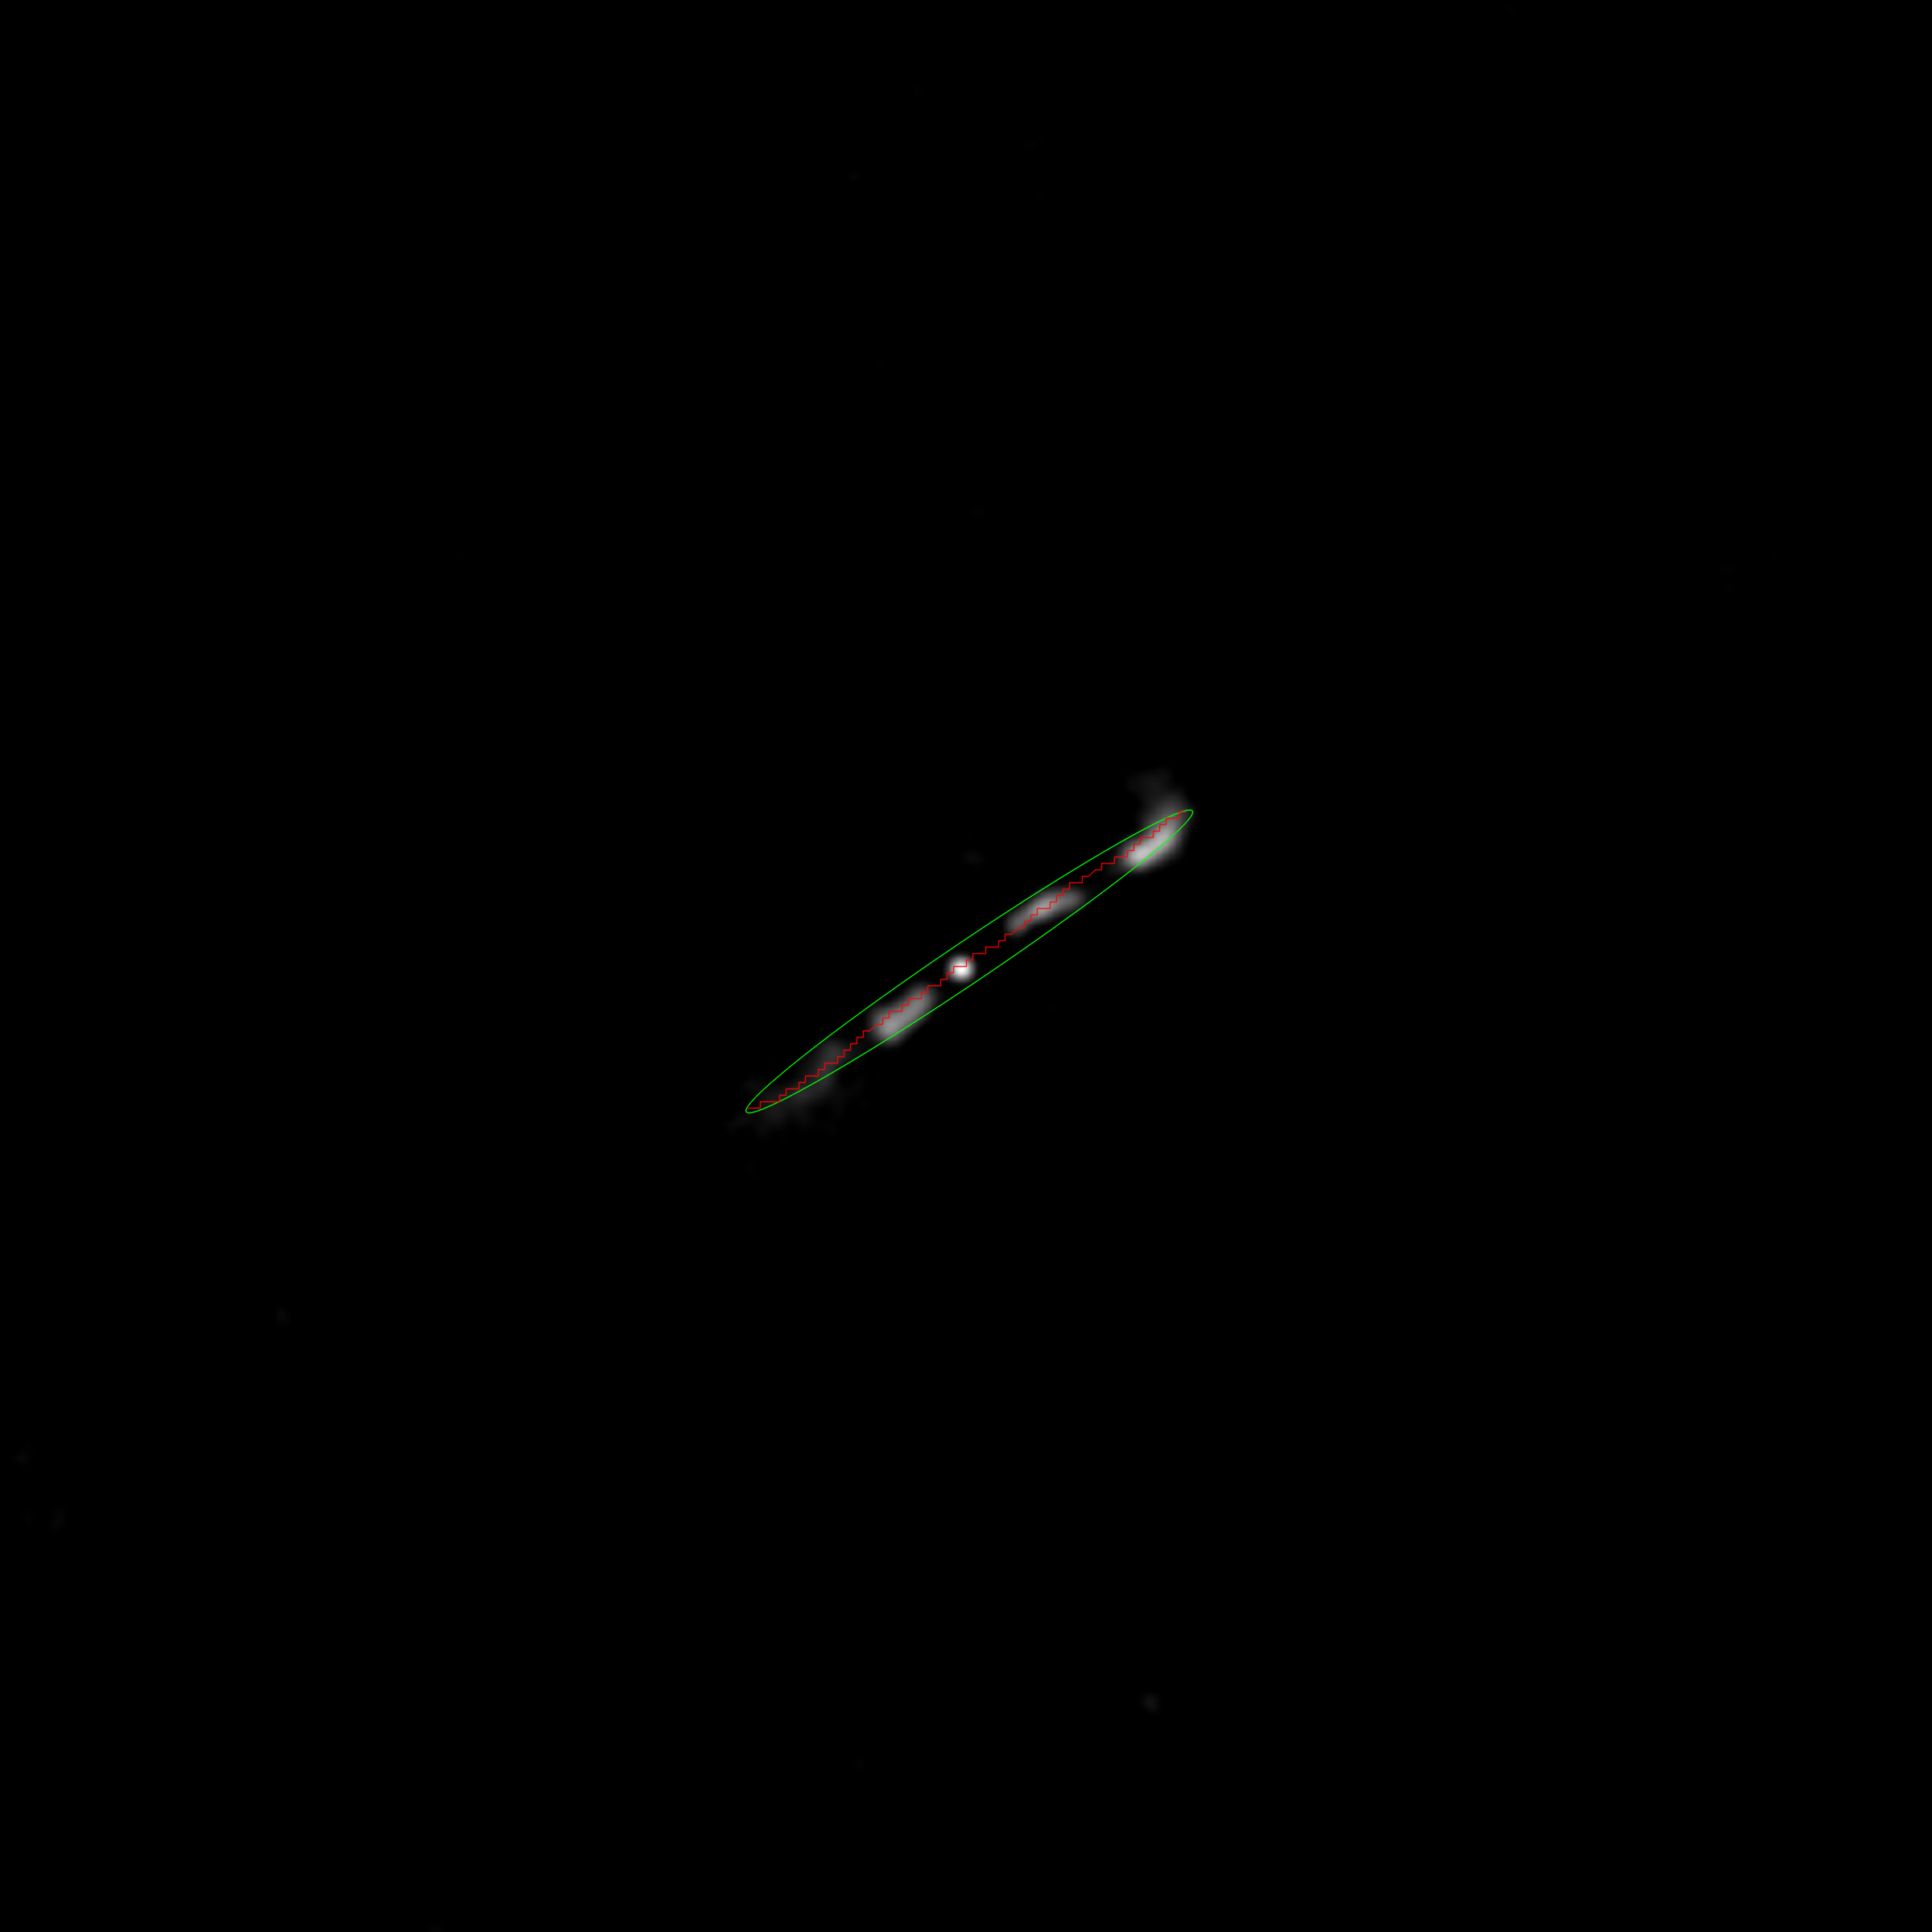
\includegraphics[clip, trim=800 800 800 800, scale=1.5, width=0.3\linewidth]{Figure/Section 3/149.318_19.114_0_MiraBest.png}
    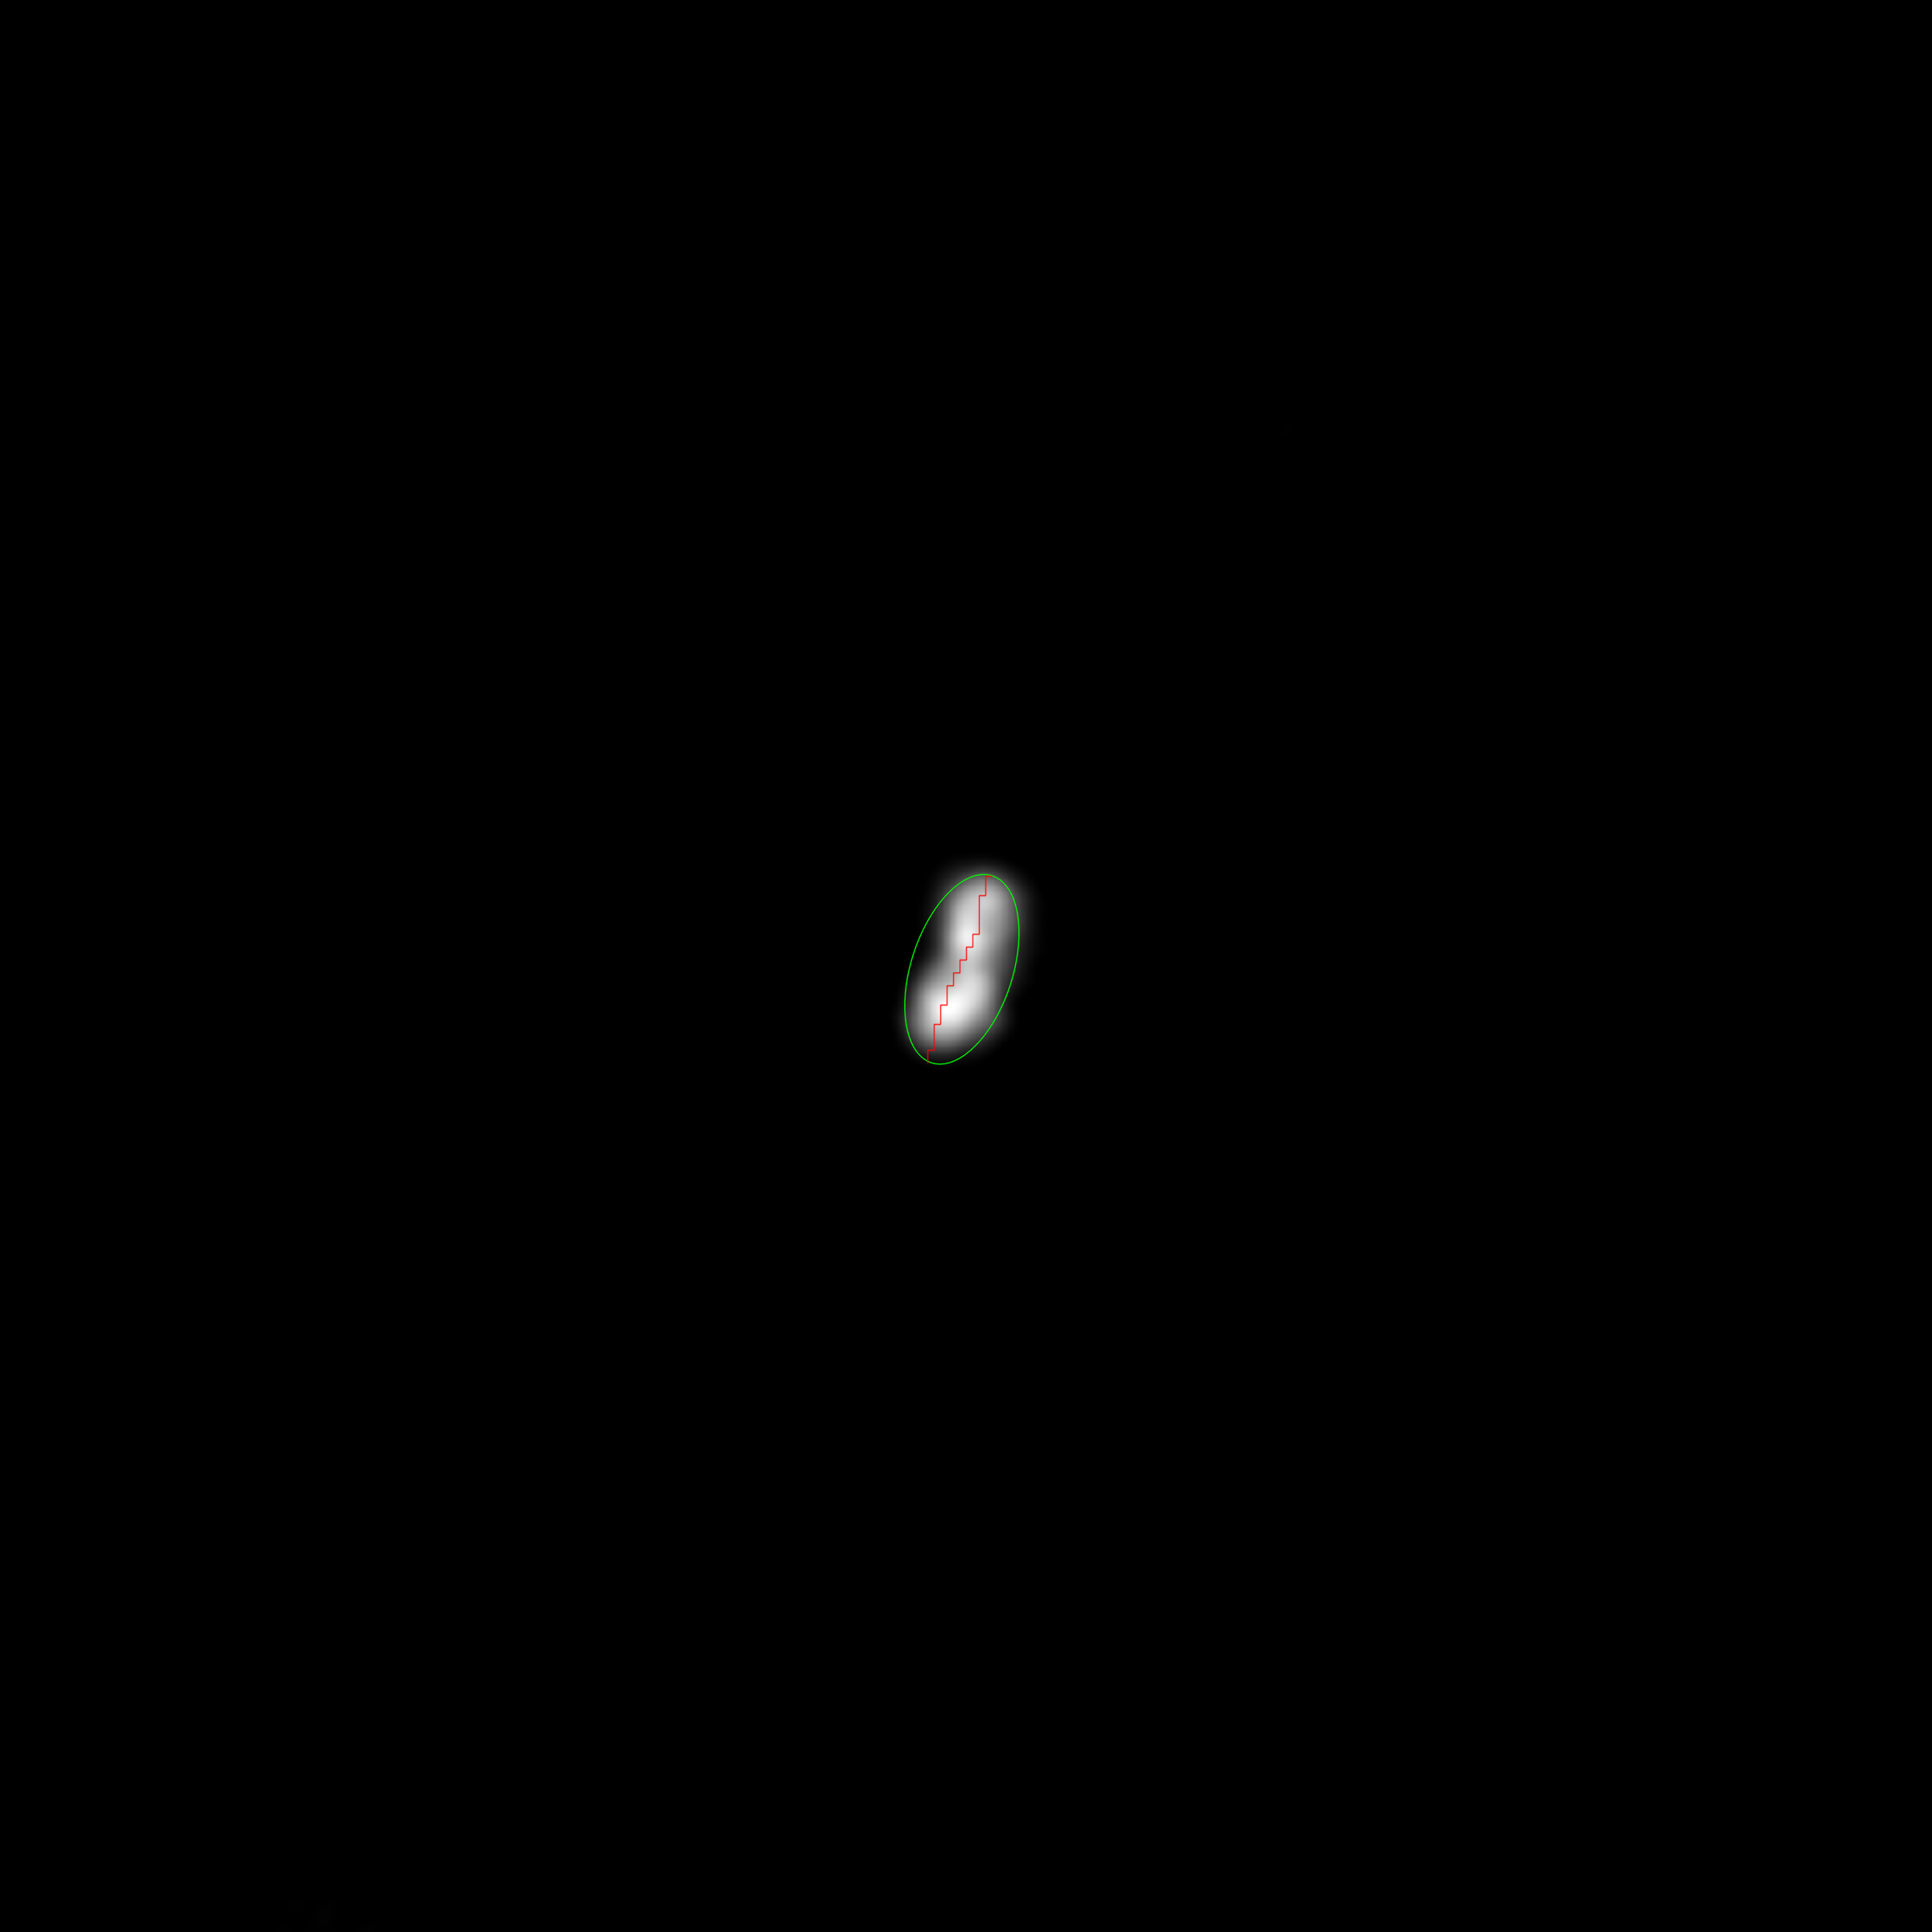
\includegraphics[clip, trim=1000 1000 1000 1000, scale=1.5, width=0.3\linewidth]{Figure/Section 3/150.738_19.865_0_Gendre.png}
    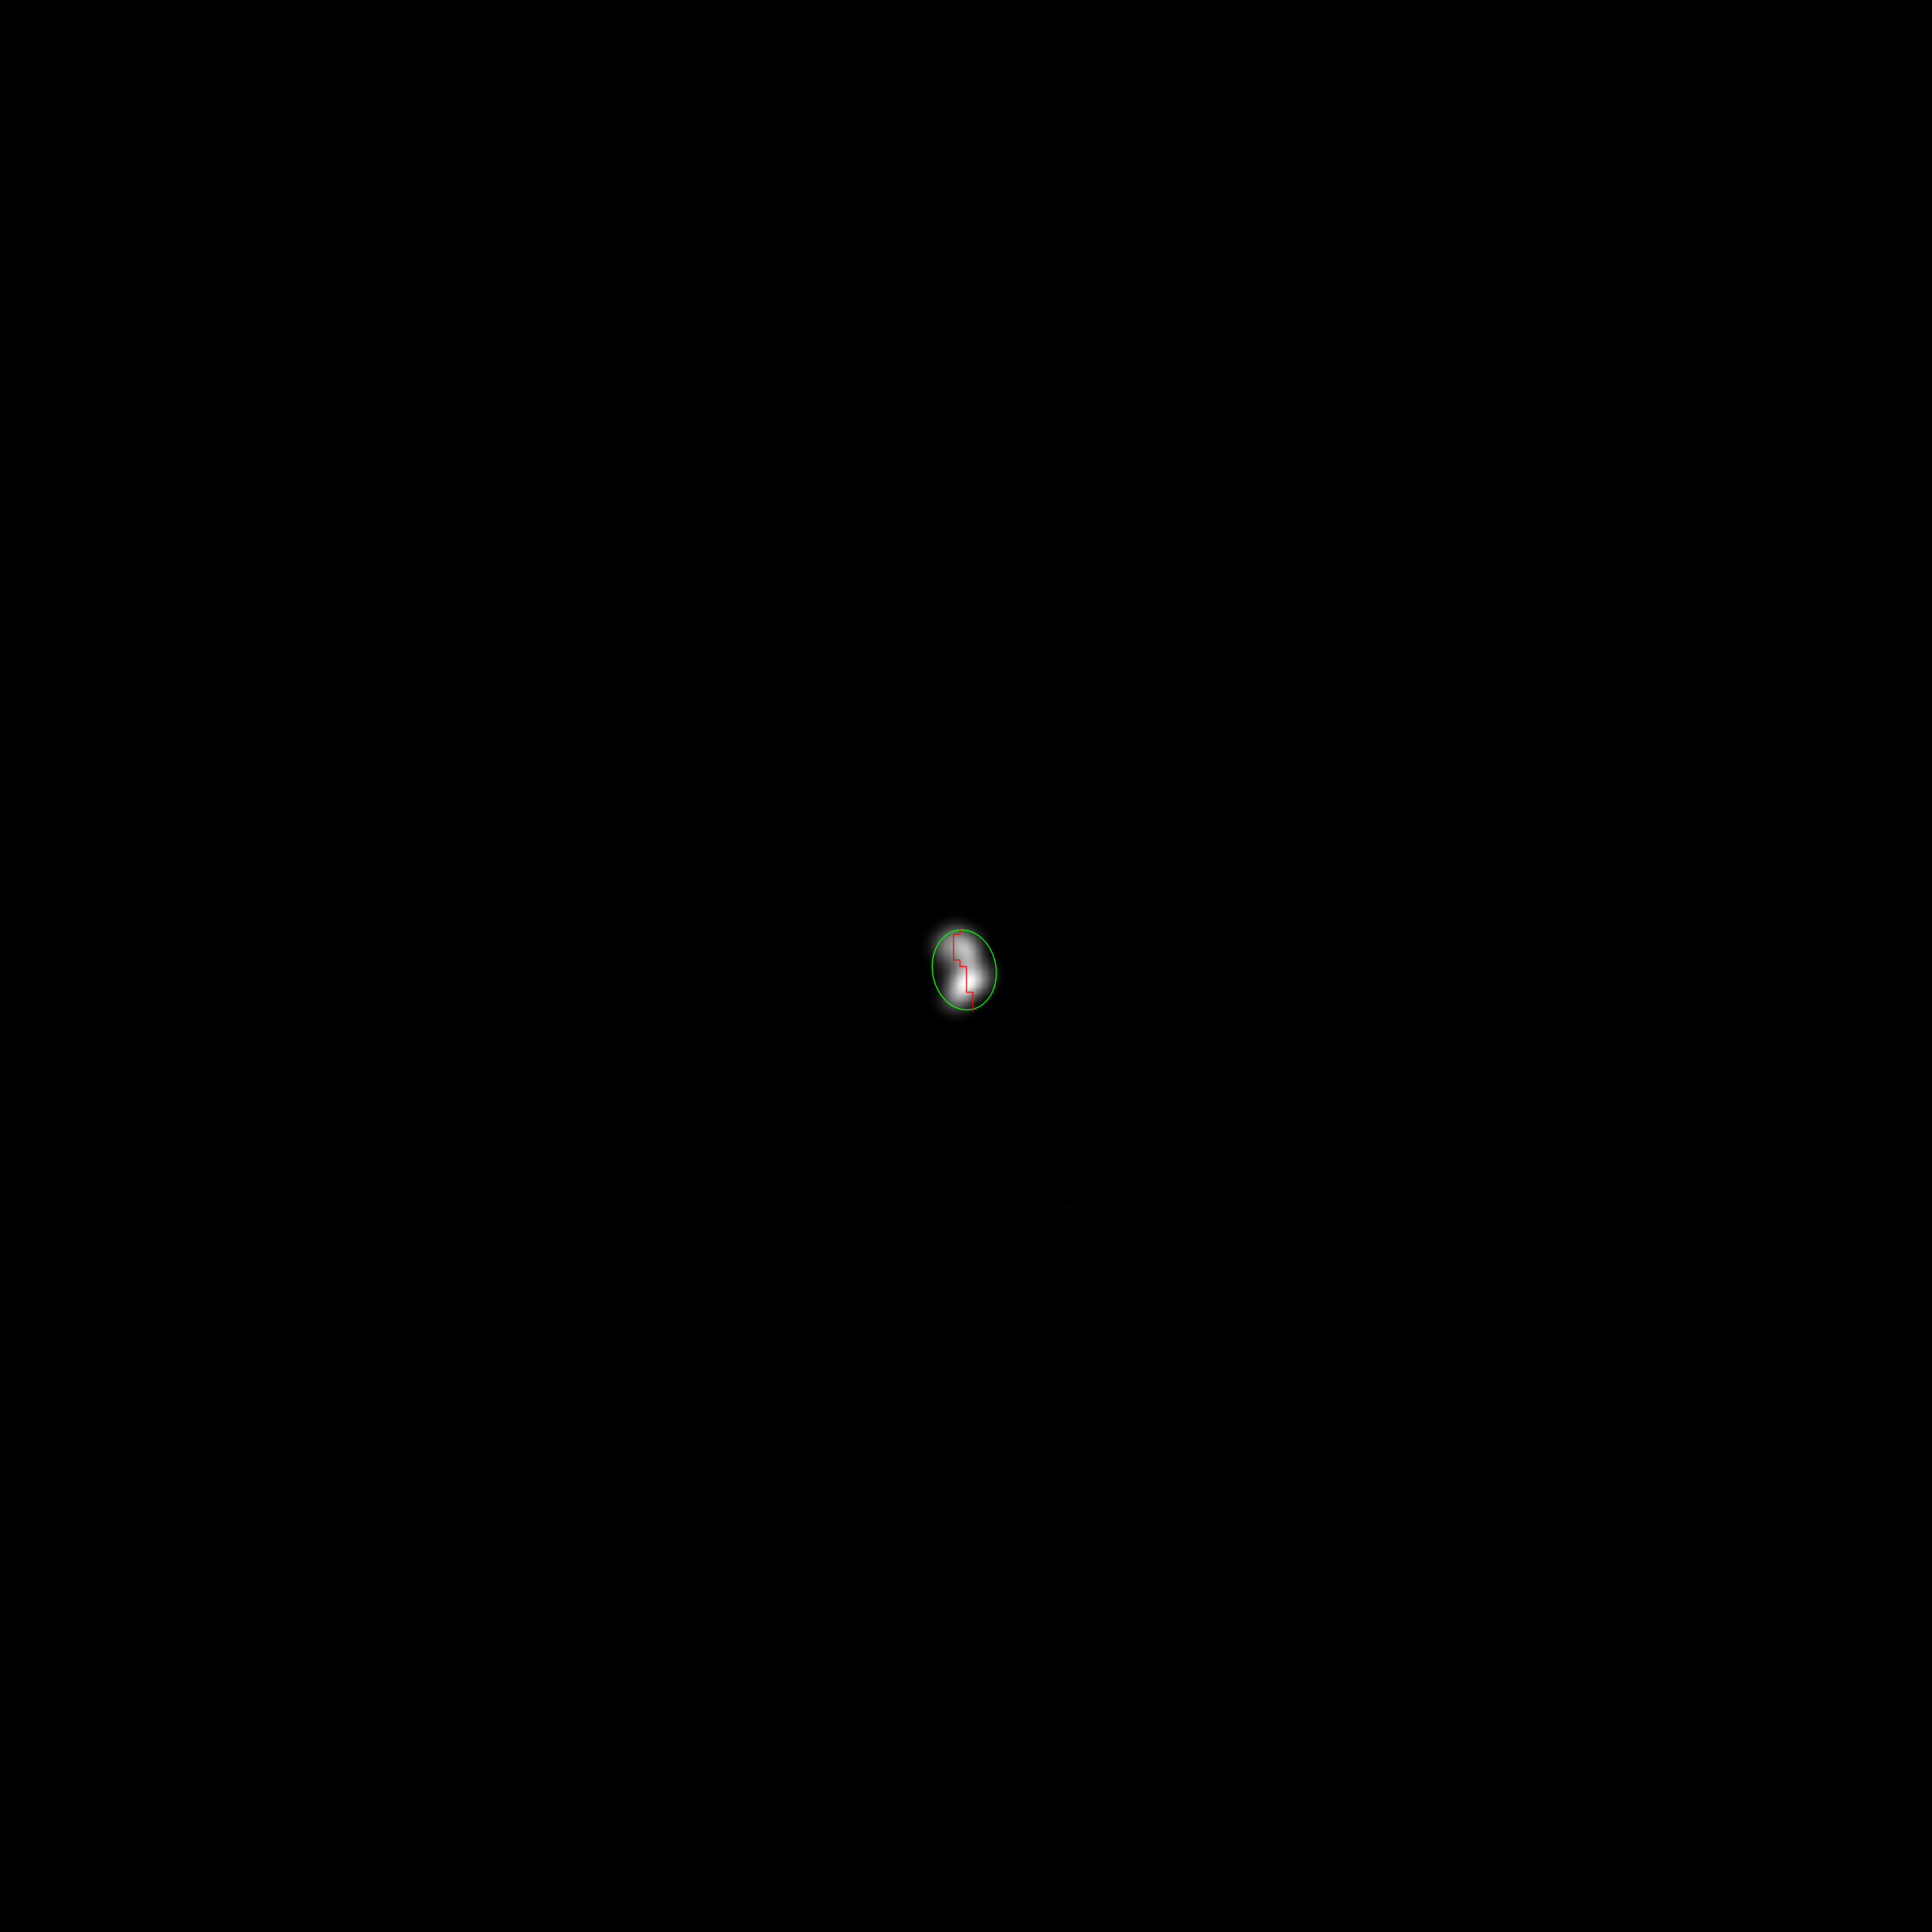
\includegraphics[clip, trim=1080 1080 1080 1080, scale=1.5, width=0.3\linewidth]{Figure/Section 3/228.764_22.529_0_Gendre.png}
    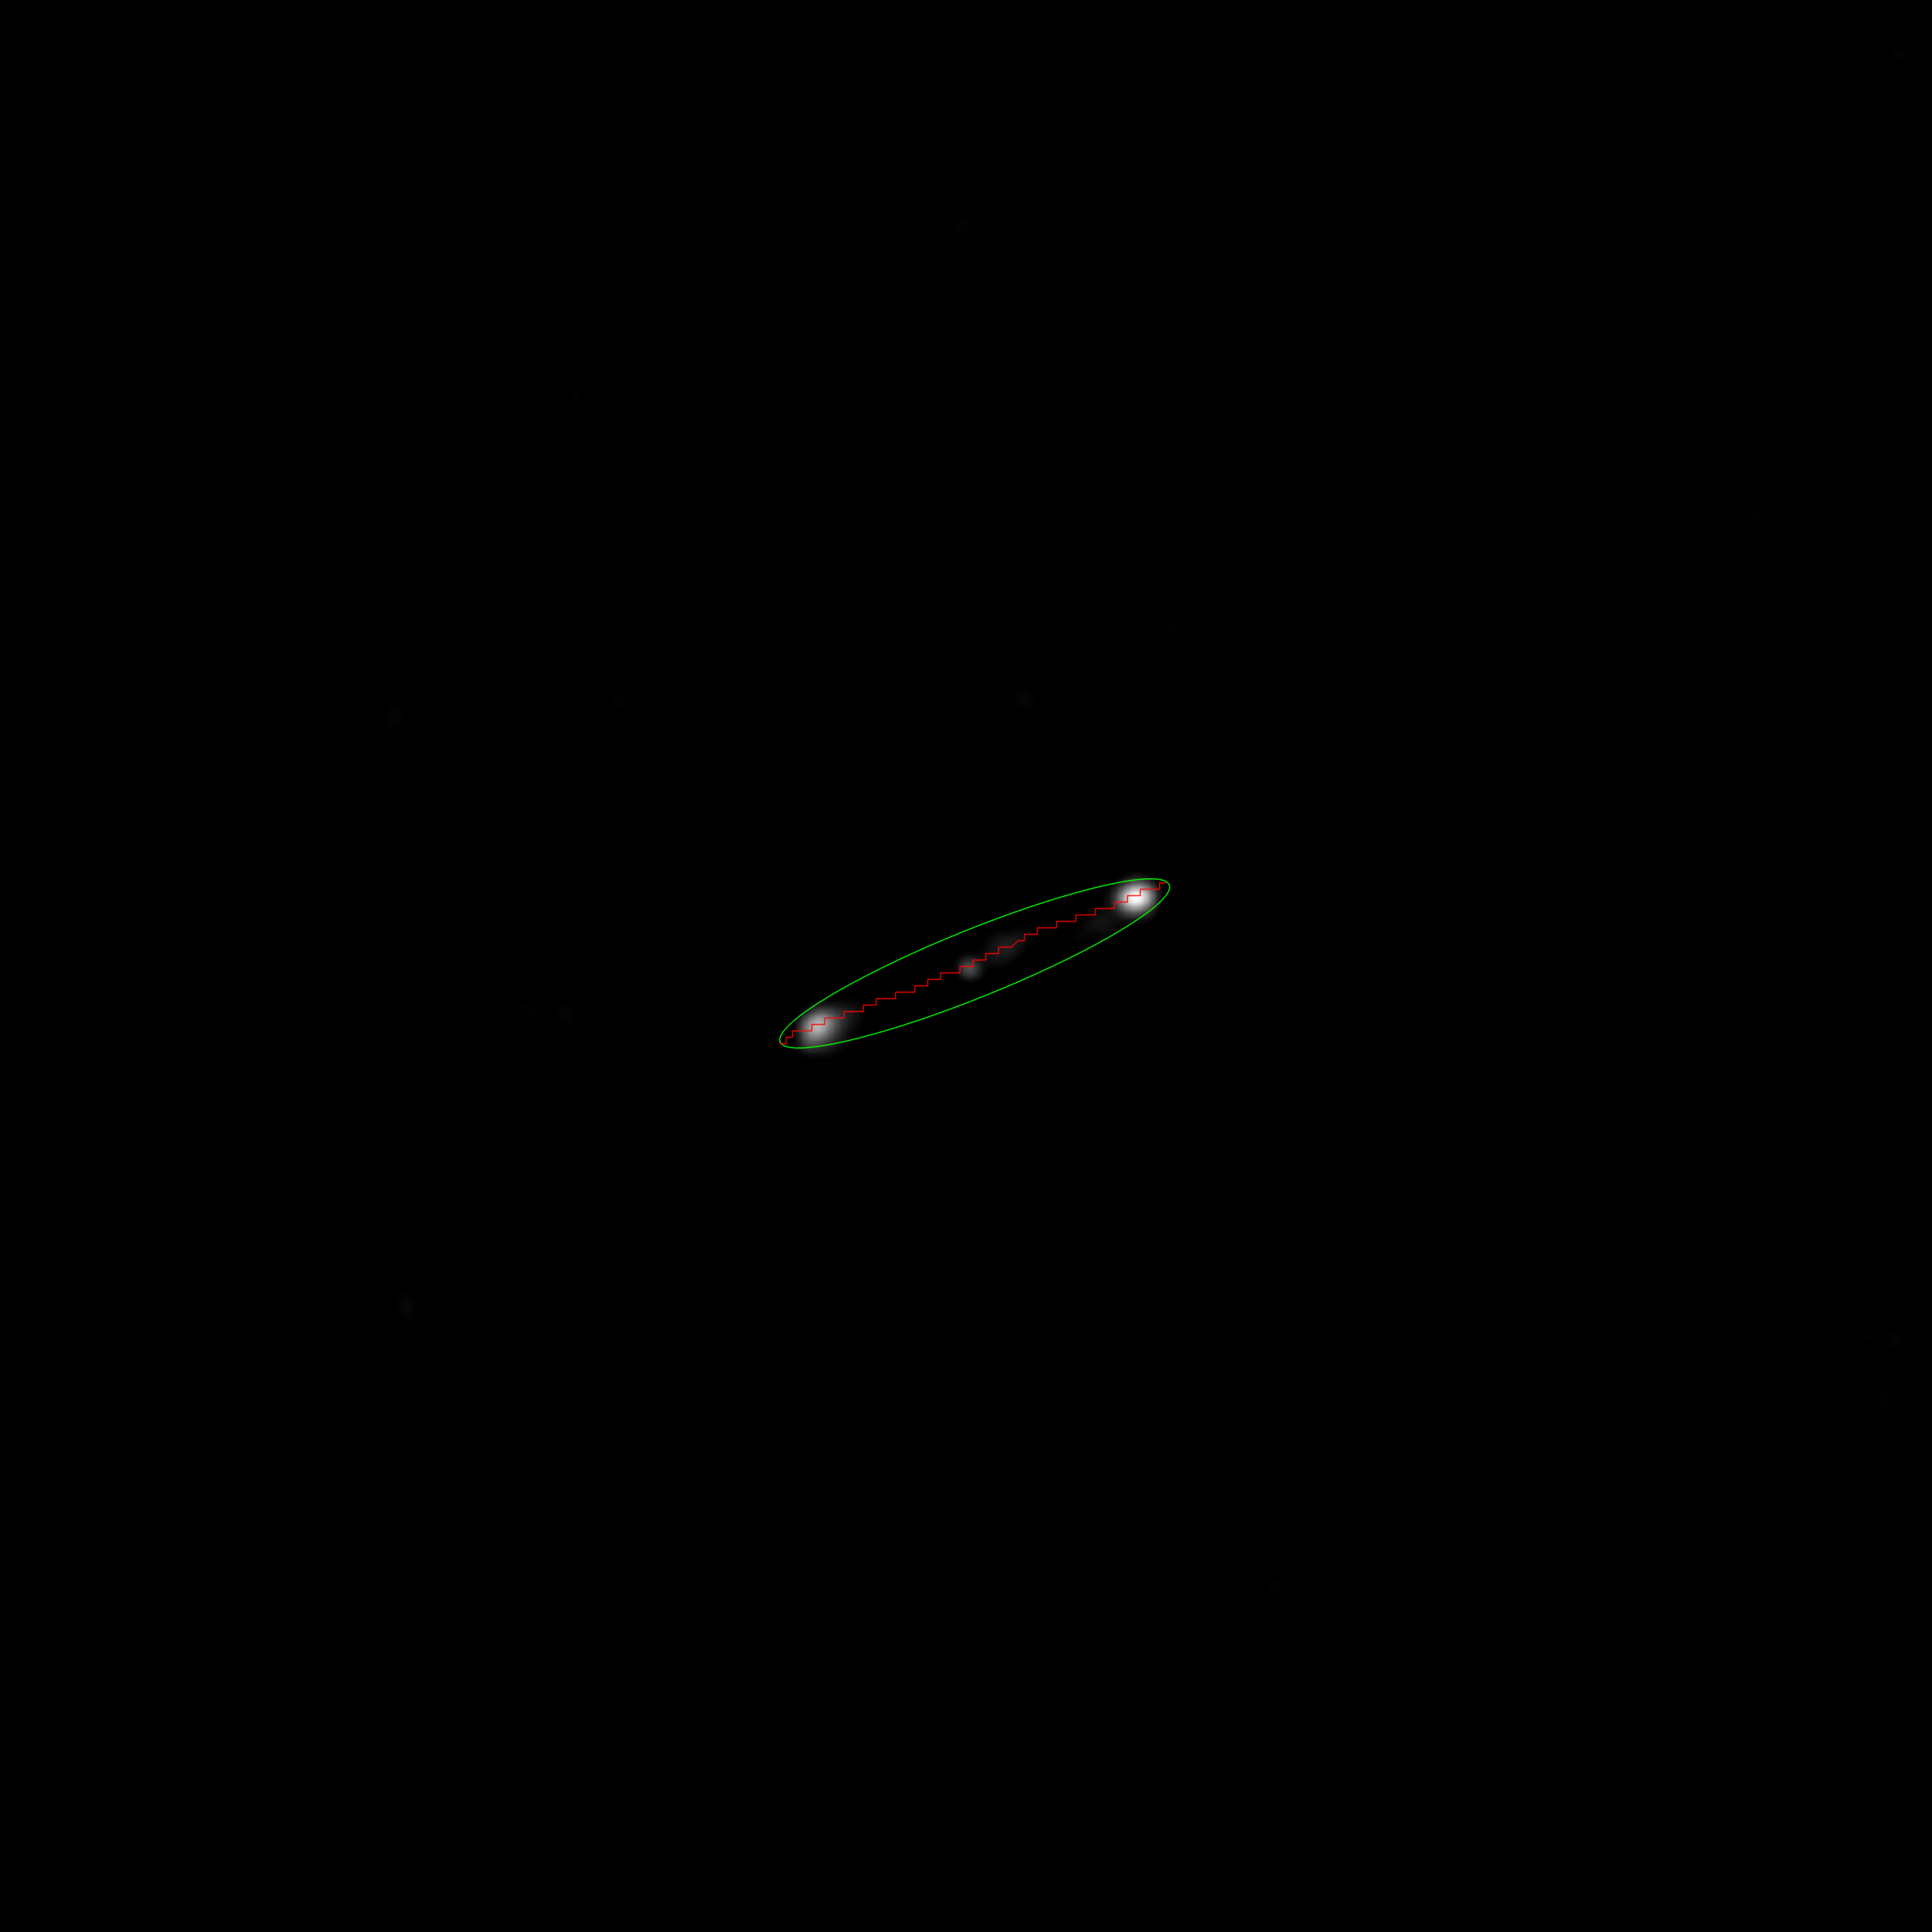
\includegraphics[clip, trim=920 920 920 920, scale=1.5, width=0.3\linewidth]{Figure/Section 3/180.424_22.946_1_MiraBest.png}
    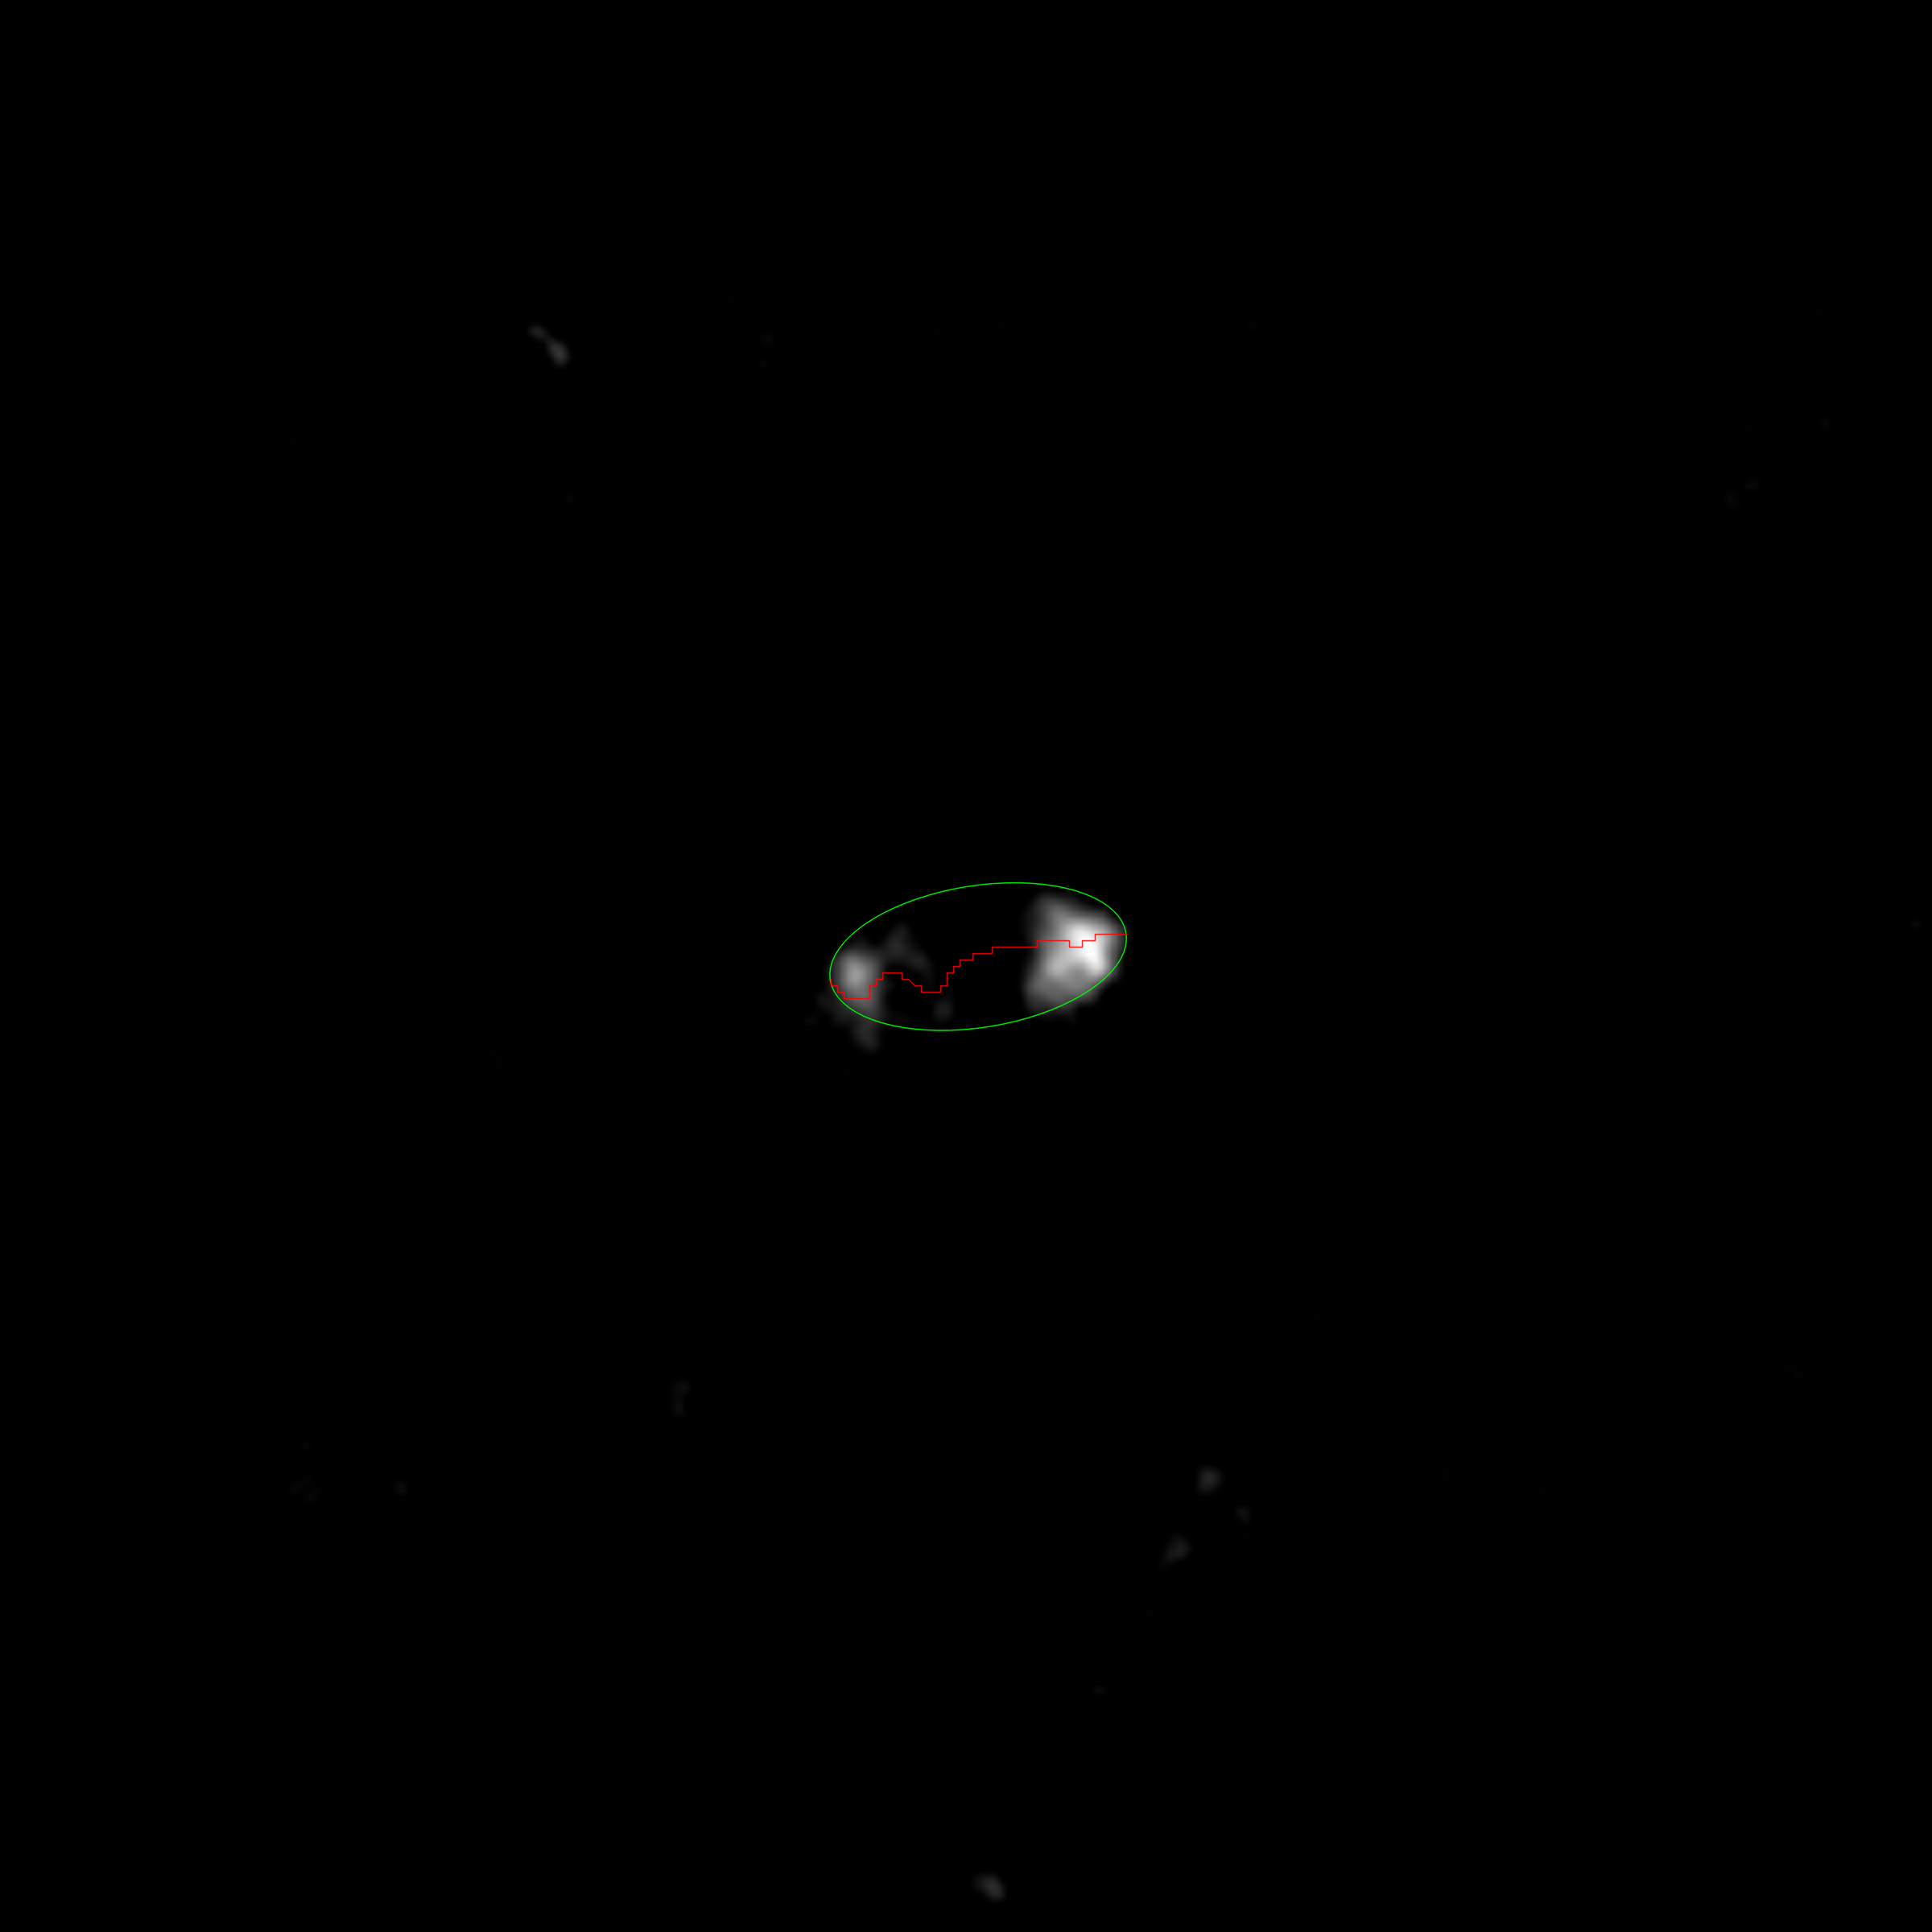
\includegraphics[clip, trim=960 960 960 960, scale=1.5, width=0.3\linewidth]{Figure/Section 3/213.728_22.633_1_MiraBest.png}
    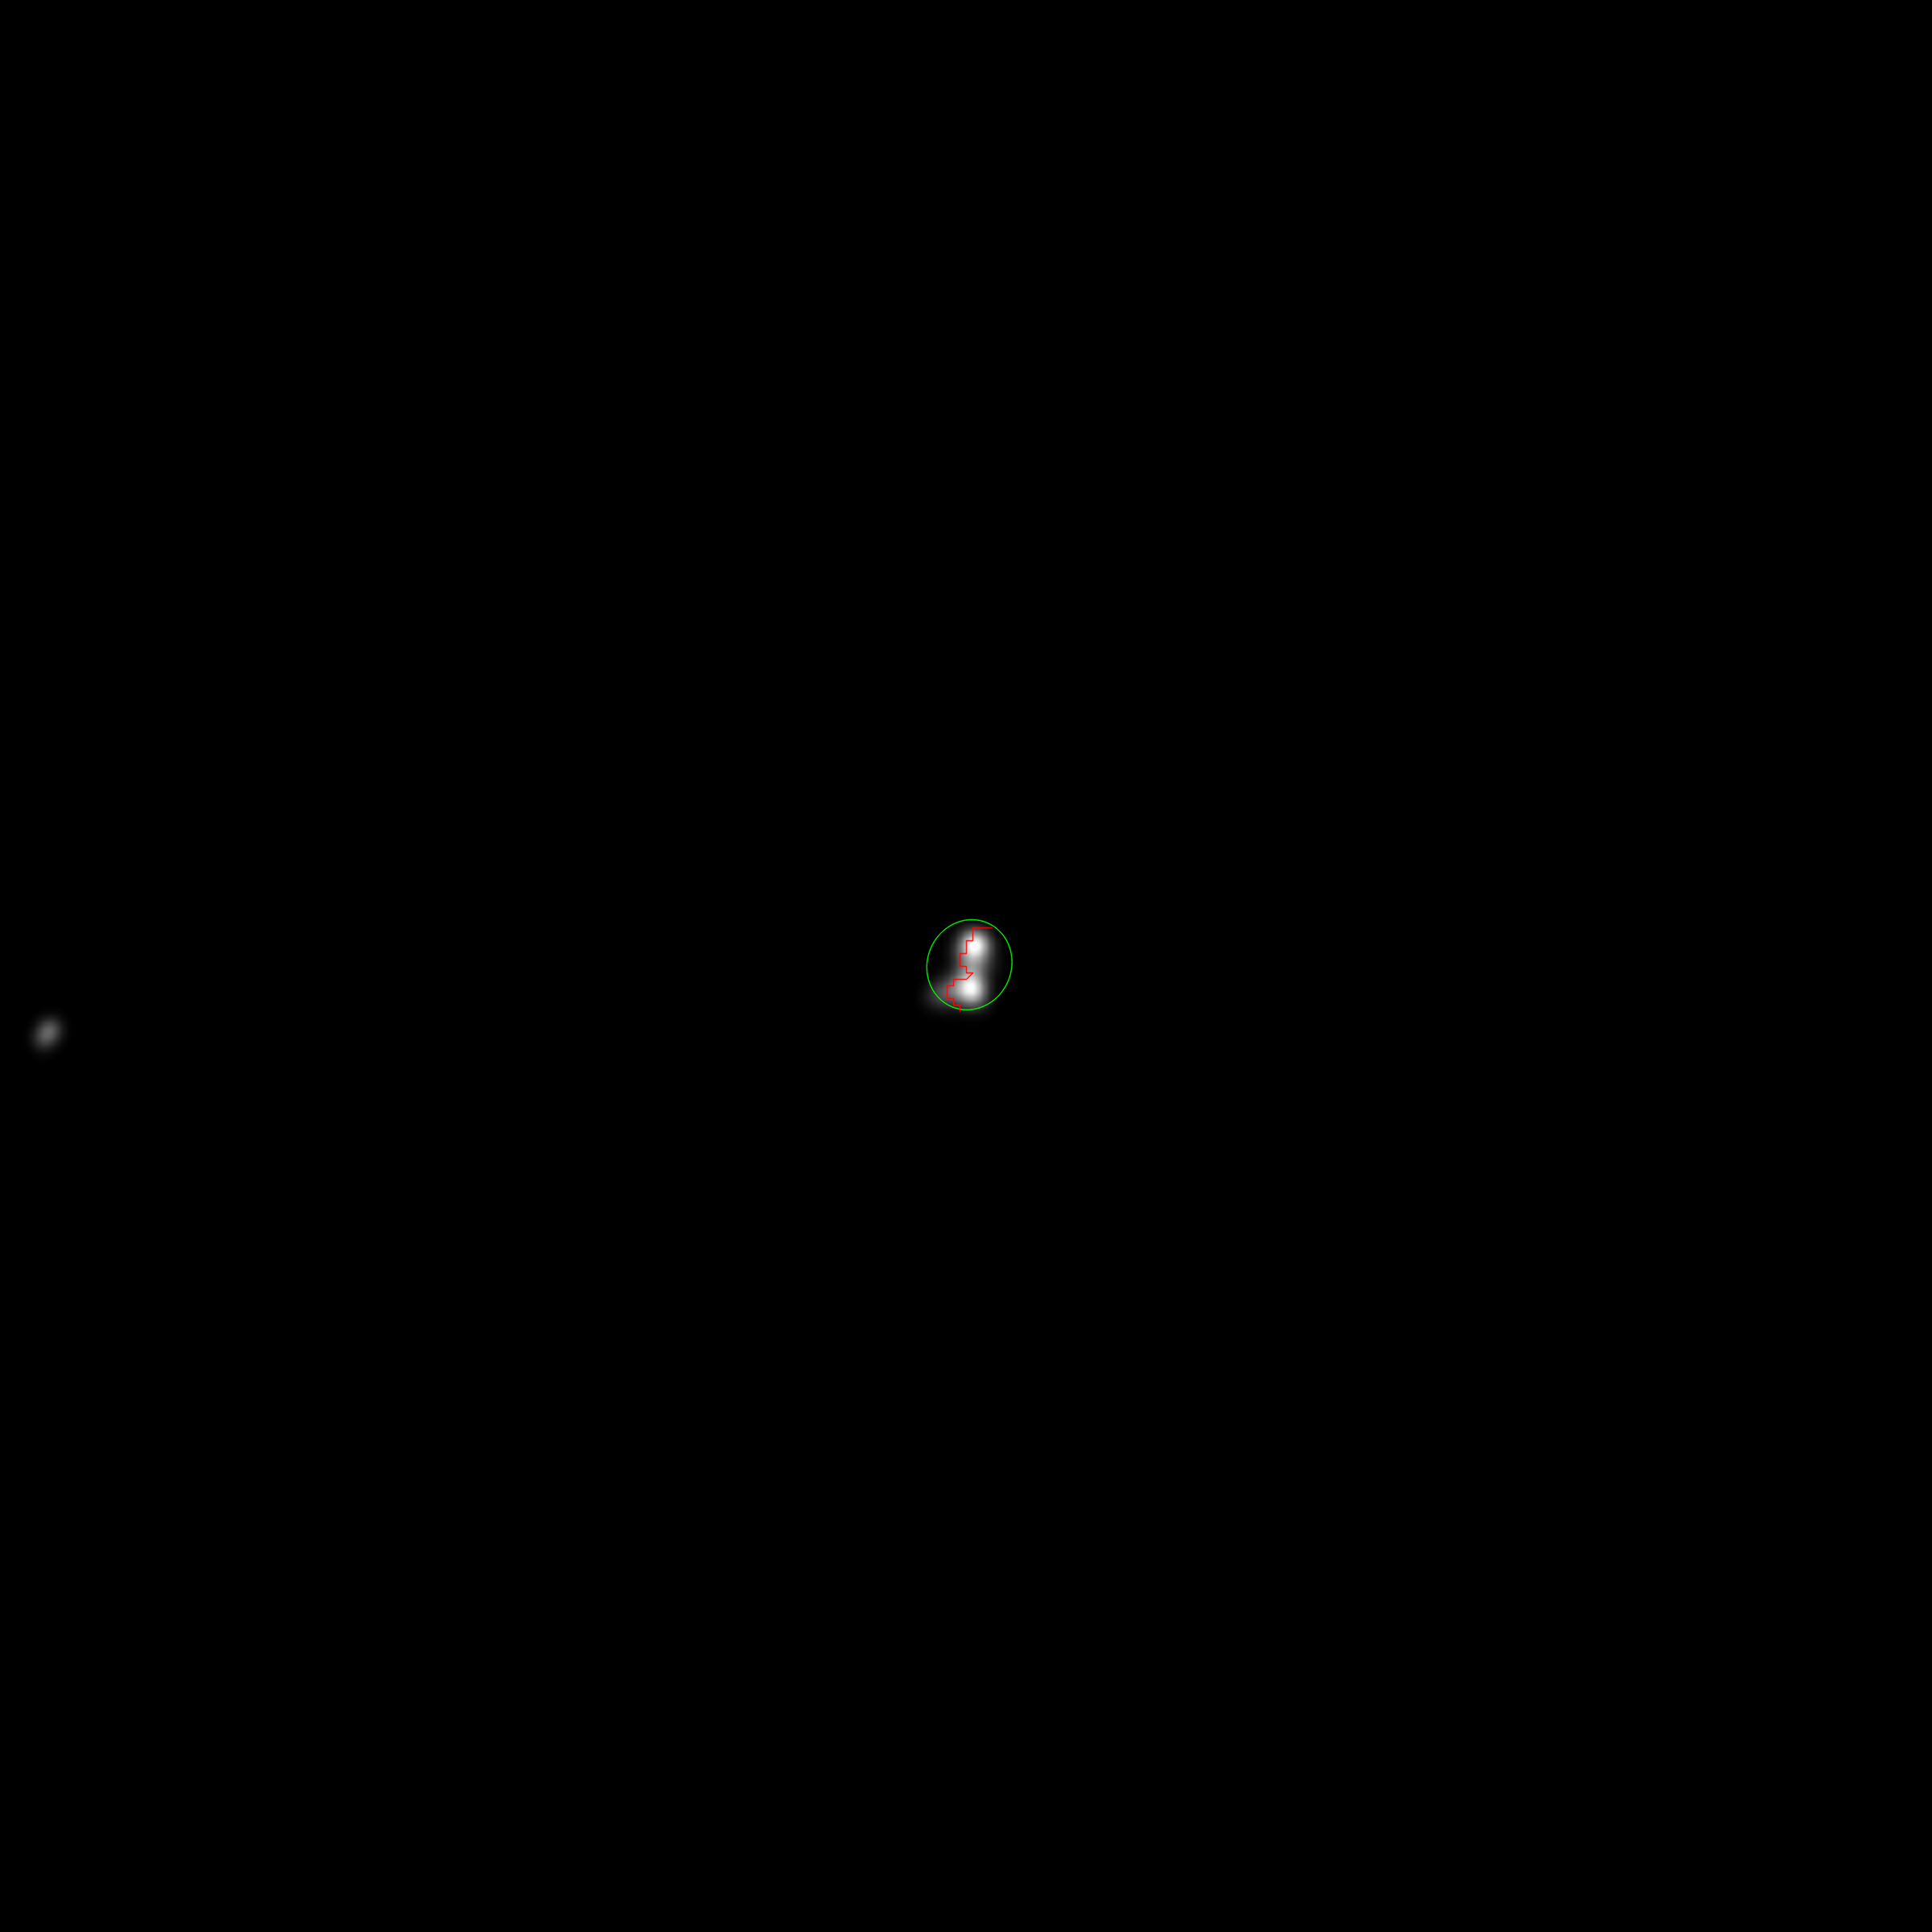
\includegraphics[clip, trim=1080 1080 1080 1080, scale=1.5, width=0.3\linewidth]{Figure/Section 3/125.391_47.043_1_Gendre.png}
    \caption{
    Top Panel: showing the FRI.
    Bottom Panel: showing the FRII.
    The green ellipse represents the algorithm-identified RG ellipse, while the red curve corresponds to the central line of the RG.
    }
    \label{fig:Figure2}
\end{figure}

\subsection{FITS flux density and centreline profiles}

For physically calibrated measurements we retrieve FIRST FITS cutouts at the source coordinates, using nearby survey tiles to fill cutout boundaries when required while retaining their world-coordinate information. The image-domain emission mask and centreline are stored together with the centre, axis, source coordinates, and redshift in a geometry file. We register this geometry against the FITS cutout before measuring the source. Earlier centreline files derived from display-image greyscale values are kept distinct from FITS-based intensity and luminosity profiles.

The FITS brightness is in \(\mathrm{Jy\,beam^{-1}}\). With beam full widths \(B_{\rm maj}\) and \(B_{\rm min}\), we use \(\Omega_{\rm beam}=\pi B_{\rm maj}B_{\rm min}/(4\ln2)\); the FITS world-coordinate scale gives the pixel solid angle \(\Omega_{\rm pix}\). Integrating over the registered source mask gives
\begin{equation}
S_{\rm int}=\sum_{i\in M} I_i\,\frac{\Omega_{\rm pix}}{\Omega_{\rm beam}},
\end{equation}
where \(I_i\) is the FITS pixel brightness and \(M\) the accepted emission mask. The local background rms and the number of independent beam areas in the mask enter the flux-density uncertainty estimate. We then compute the rest-frame monochromatic luminosity using the implemented spectral-index convention,
\begin{equation}
L_{\nu}=\frac{4\pi d_{\rm L}^{2}S_{\rm int}\,10^{-26}}{(1+z)^{1-\alpha}},
\end{equation}
with \(S_{\rm int}\) in Jy, \(L_{\nu}\) in \(\mathrm{W\,Hz^{-1}}\), \(\alpha=0.75\), and luminosity distance \(d_{\rm L}\) in metres. We adopt a flat cosmology with \(H_0=67.74\,\mathrm{km\,s^{-1}\,Mpc^{-1}}\) and \(\Omega_{\rm m}=0.3089\). Missing redshifts or unusable FITS data do not yield a luminosity measurement.

Along the ordered centreline we record signed distances from the host and sample both the local FITS brightness and a beam-weighted transverse profile. The derived luminosity profiles are expressed separately from their \(\mathrm{Jy\,beam^{-1}}\) samples and from the older greyscale profiles. For comparisons of central and outer emission, the centreline is partitioned about the host into a central segment and two sides; central-to-outer peak and integrated-profile ratios are calculated only when the requisite segments and measurements are available. \autoref{fig:CentralLine} illustrates the profiles.

\subsection{Optical properties and quality control}

We join the selected NED counterparts to catalogued coordinates and redshifts, and query VizieR and SIMBAD for available black-hole and host-galaxy mass estimates. Measurements from heterogeneous catalogues are cleaned and converted to consistent mass units before a representative median is written to the combined source table. We retain missing masses as missing values rather than inferring them from the radio images. The optical, image-domain, and FITS outputs are cross-matched by source identity, with separate checks on counterpart ambiguity, mask and centreline quality, FITS coverage, and valid redshift. The resulting subsets used for each comparison may therefore differ. The available redshift and mass distributions are shown in \autoref{fig:Redshift&MassDistribution}.

\begin{figure*}[!htbp]
    \centering
    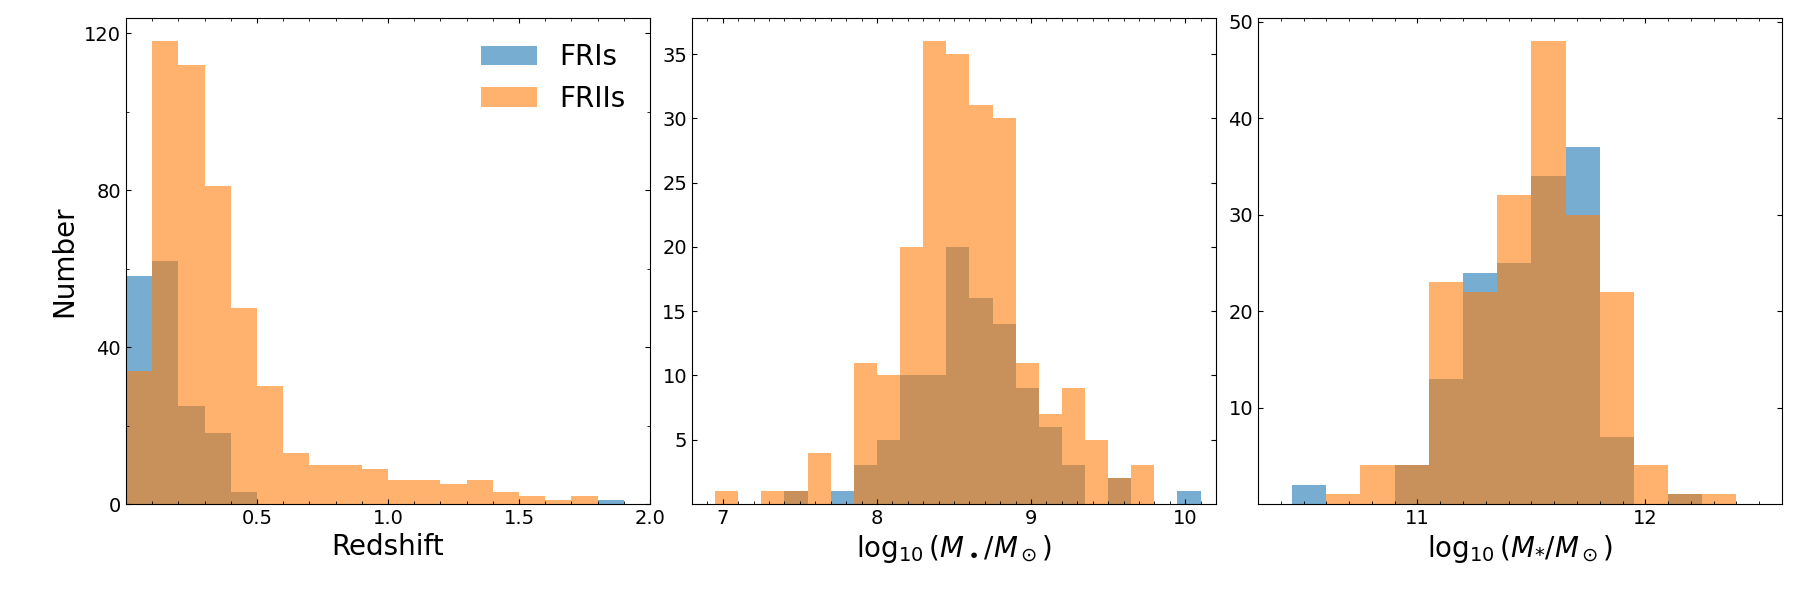
\includegraphics[width=0.9\linewidth]{Figure/Section 3/Redshift&MassDistribution.png}
    \caption{Redshift, central black-hole mass, and host-galaxy stellar-mass distributions for the visually screened sample with available counterpart information (FRIs in blue; FRIIs in orange). From left to right, the panels contain 169 FRIs and 506 FRIIs, 101 FRIs and 217 FRIIs, and 147 FRIs and 192 FRIIs, respectively. Mass estimates are compiled from the available catalogued measurements for each counterpart.}
    \label{fig:Redshift&MassDistribution}
\end{figure*}



%\subsection{Flood-filling Algorithm}\label{sec:Section3_3}
%To extract the contours of RGs, employing the Flood-filling algorithm serves as an effective method for determining the extent of the associated RG \citep[e.g.,][]{mingo_revisiting_2019,hales_blobcat_2012}; Starting from known internal points, the Flood-filling algorithm only expands to adjacent non-boundary points, while boundary points are consistently excluded; this facilitates the identification of the contours of RGs under specific conditions \citep{lieberman_how_1978,fishkin_family_1984}. In this procedure, it is specified that the Flood-filling algorithm will disperse seed points in all connected regions of the image with non-zero brightness, while the brightness threshold is set to 5\% of the brightness value of the brightest point in the image.


%\subsection{Principal Component Analysis}\label{sec:Section3_4}
%Most applications of PCA in astronomy relate to identifying eigenvectors across a population of objects \citep[e.g., PCA tomography][]{steiner_pca_2009}, PCA will be employed to detect the principal direction that best align with RG structures in the context of the present work. PCA is a powerful technique for extracting structure from potentially high-dimensional datasets, and a small number of principal components is often sufficient to account for most of the structural information in the data \citep{hofmann_kernel_2008}. Specifically, for the morphological analysis of RGs\textemdash whose observational data typically encompasses multidimensional information (e.g., spatial coordinates and brightness gradients)\textemdash PCA integrates these discrete data points into a low-dimensional principal component space. It prioritizes and preserves the information driven by the highest variance while filtering out noise and redundant signals unrelated to morphology. In this paper, in addition to the targeted RGs, other radio sources (e.g., compact sources) present in the acquired FIRST images interfere with the processing of the target. Compared with RGs, these interfering sources exhibit simpler structures and significantly smaller scales. Consequently, when PCA is employed to process the brightness distribution, the variance corresponding to the identified largest distribution direction is substantially greater than that of the second largest variance. PCA enables the direct retrieval of the core morphological features of RGs without relying on complex auxiliary data, which aligns with the previously outlined requirement for efficient and concise morphological extraction.


%The Central Line derived via skeletonization is proposed as a structural reference for RG systems. PCA aids in identifying representative clumps; however, these clumps cannot be readily interpreted as the full RG system, and their structural validity requires further verification. The processed central-line structure is illustrated in \autoref{fig:Redshift&MassDistribution}. After excluding significant deviations, the most complete RG system structures and their associated optical counterpart information are retained.

%Skeletonization is a well-established method for image structure characterization, and Breadth-First Search (BFS) enables the identification of the central line of RG skeleton\textemdash this line, in turn, facilitates the simplification of the features of the RG's brightness distribution. Skeletonization enables efficient compression of RG structure while preserving its core structural information. Specifically, using iterative skeletonization methods, foreground regions can be reduced to single-pixel-wide skeletons while maintaining topological features; for analogous work, see \cite{vardoulaki_fr-type_2021}. Then, BFS algorithm enables the identification of a line within the skeletonization process that characterizes the center of RG brightness distribution. This constitutes a pruning process, as extraneous branches in the skeleton are irrelevant for characterizing the overall orientation of lobe structures. Thus, BSF algorithm can retain the primary backbone\textemdash most representative of lobe structure\textemdash hereafter referred to as the central line. Merely applying BFS algorithm alone is insufficient; it is additionally required to incorporate into the algorithm the constraint that the direction of the central line is roughly aligned with the PCA-derived principal direction, as well as the requirement that the central line passes through hot spots or other compact clumps.

%Notably, \cite{barkus_application_2021} employed analogous methodologies; however, their ridge lines \textemdash developed primarily for the identification and morphological classification of extended radio galaxies in radio astronomy  \textemdash may be less well-suited to RG systems featuring large structural gaps or curved head-tail configurations.


\begin{figure}[!htbp]
    \centering
    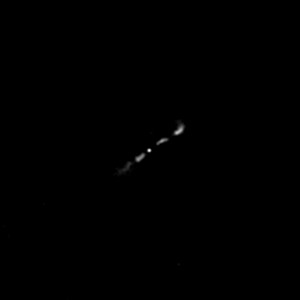
\includegraphics[clip, trim=100 100 100 100, scale=1.5, width=0.45\linewidth]{Figure/Section 3/origin_149.318_19.114_0_MiraBest.png}
    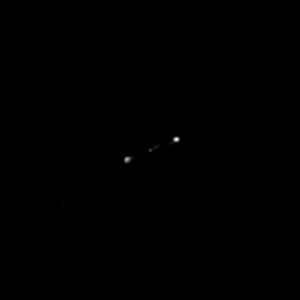
\includegraphics[clip, trim=100 100 100 100, scale=1.5, width=0.45\linewidth]{Figure/Section 3/origin_180.424_22.946_1_MiraBest.png}
    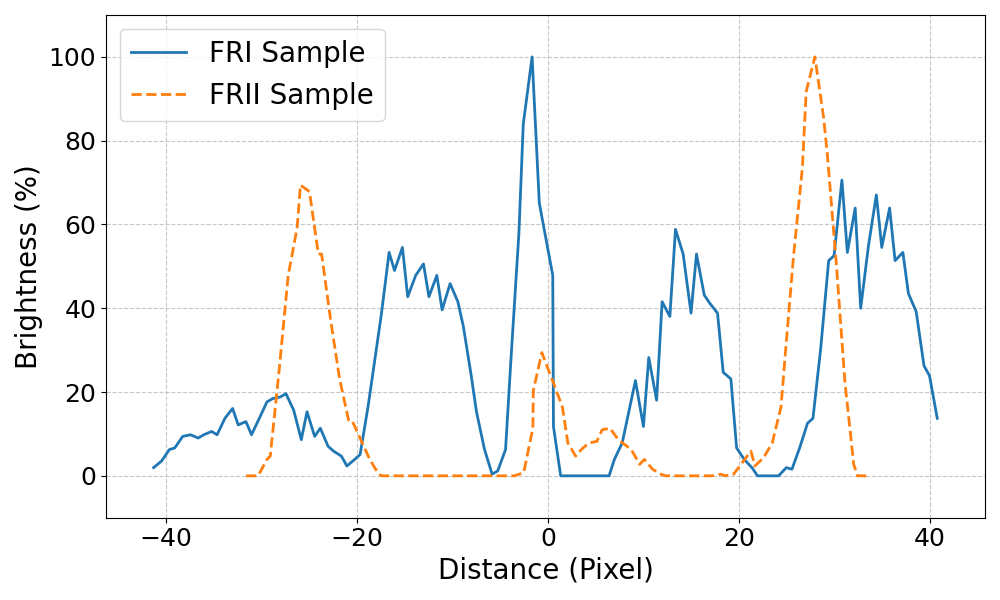
\includegraphics[width=1\linewidth]{Figure/Section 3/CenterLineLuminosity.png}
    \caption{Top left: FRI's sample (R.A. 149.318°, Dec. 19.114°);  Top right: FRII's sample (R.A. 180.424°, Dec. 22.946°);  Bottom: Luminosity distribution along the central line, with the peak brightness normalized to 100\%.}
    \label{fig:CentralLine}
\end{figure}



% 在这一方面的方法中，椭圆很重要，过去曾经有不少工作都用了椭圆结构
%Elliptical structures hold substantial significance in morphological studies of radio galaxies (RGs). A simple elliptical morphology has been repeatedly observed in prior analyses of RG structure \citep[e.g.,][]{lin_new_2024, carilli_cygnus_1996, begelman_overpressured_1989}. Evidently, elliptical structures serve as a general and effective descriptor for radio-loud sources.


%To enable independent modeling of the core region and lobes of RGs, \cite{lin_populations_2010} defined \(S\) as the angular separation between the peaks of highest surface brightness on either side of the host galaxy, designating \(T\) as the total linear size of the RG and thus defining \(r_s \equiv S/T\) as the primary metric for RG morphology. A key component of this approach involves fitting source components via Gaussian modeling; unfortunately, many sources in the dataset used in this study lack beam parameters consistent with those in the FIRST Catalog.
%To enhance the universality of the simulations, the methodology is simplified herein: 
%For FRIIs, hot spots are identified by locating the brightest points and outermost elliptical Gaussian components on opposite sides of the RG’s optical counterpart. Meanwhile, \(T\) is adopted as the maximum distance between the outermost pixels of the RG, a parameter that characterizes the overall size of the system. 
%For FRIs, \(S\) is defined as the major-axis size of the largest elliptical Gaussian component at the system’s center.


%Elliptical Gaussian models are fitted sequentially to decompose Gaussian components within the RG system. The process starts with an optimal single-component Gaussian fit; the modeled emission is subtracted from the original image, and fitting iterations continue on the residual image until at least 95\% of the brightness distribution is accounted for.
%Specifically, to optimally cover the entire RG, distinct strategies are adopted for different FR types. For FRI sources \textemdash featuring a bright core and the classic lobe–core–lobe morphology \textemdash a three-component elliptical Gaussian model is used to fit the central clump, decomposing it into one core and two lobes: the component with the highest brightness weight is designated as the core, and the other two as lobes. A minimum enclosing ellipse is then determined, tangent to the elliptical extents of the two lobes. For FRII sources, the RG ellipse is defined using elliptical Gaussian models of the hotspots: with the major-axis orientation fixed to the principal component direction, a minimum enclosing ellipse tangent to the hotspot elliptical boundaries is constructed.
%Ultimately, a minimum ellipse that optimally encloses the entire RG is identified for each FR type based on their distinct morphological structures.


%The process outlined above is illustrated in \autoref{fig:Different_rs}. Meanwhile, \autoref{fig:Figure2} specifically presents the elliptical structure derived from the processing workflow shown in \autoref{fig:FR_type_operate}. The equatorial coordinates (R.A. , Dec.) of these radio galaxies are as follows: (149.318°, 19.114°), (150.738°, 19.865°), (175.545°, 55.458°), (180.424°, 22.946°), (213.728°, 22.633°), (125.391°, 47.043°).


\begin{figure}[!htbp]
    \centering
    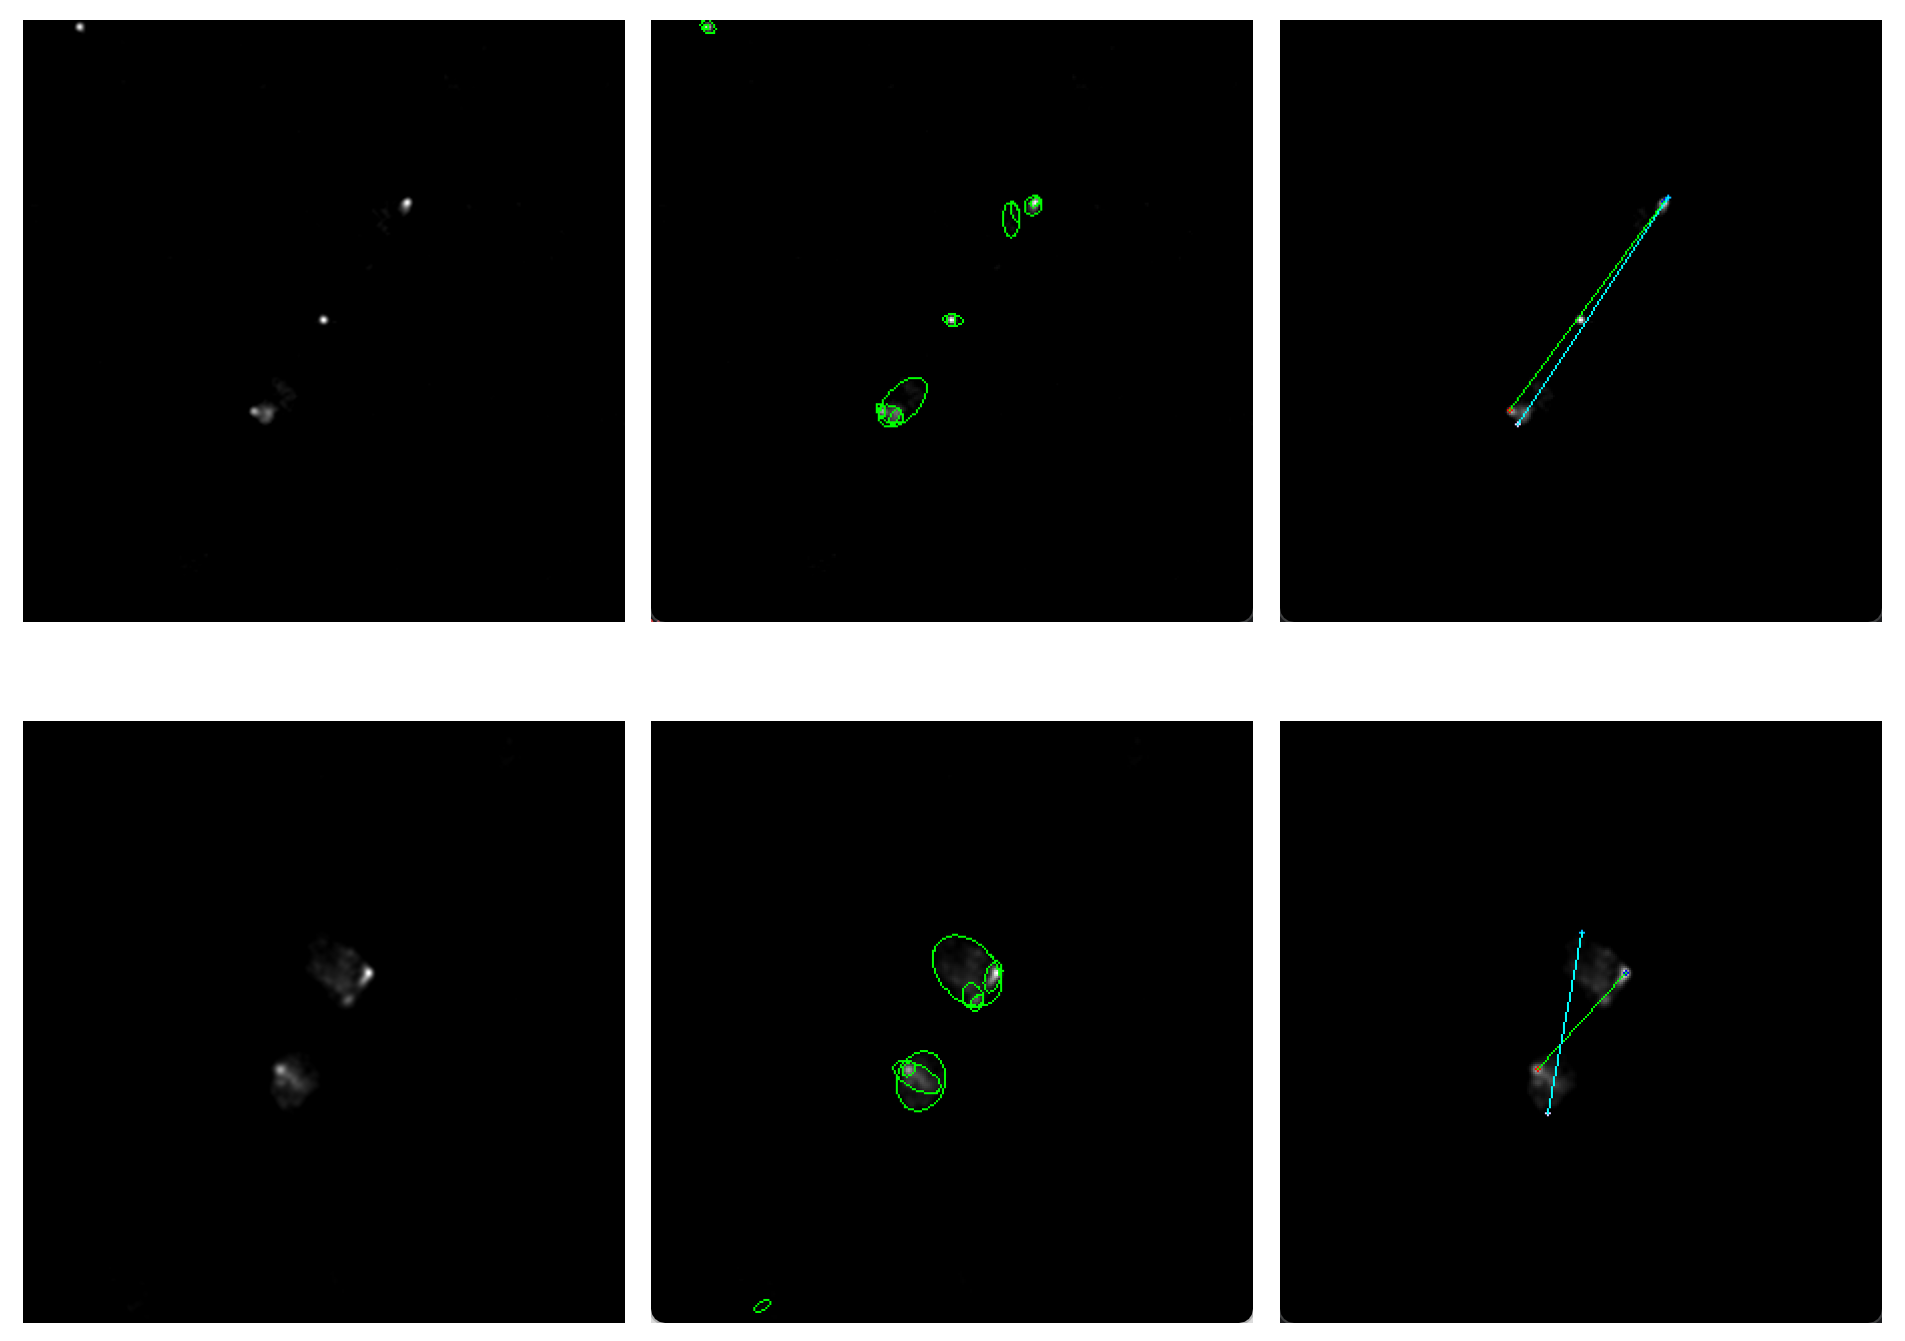
\includegraphics[width=0.9\linewidth]{Figure/Section 3/Different_rs.png}
    \caption{The first column showcases the FRII at equatorial coordinates (R.A. 155.486°, Dec. 14.725°), while the second column displays the FRII at coordinates (R.A. 148.58°, Dec. 27.267°).}
    \label{fig:Different_rs}
\end{figure}


\section{Result}\label{sec:Result}    

\subsection{The Relationship of Physical Properties}\label{sec:Section4_1}

% 统计红移和质量特征
Previous work has characterised the distribution properties of RGs. As demonstrated by the redshift distribution in \autoref{fig:Redshift} and the mass distribution in \autoref{fig:Redshift&MassDistribution}, RGs exhibit prominent clustering characteristics. When extreme outliers are excluded to focus on the overall population trends, FRIIs occupy a markedly broader distribution range than their FRI counterparts. Regarding redshift, FRI populations are predominantly confined to $z \geq 0.5 $, while FRIIs extend to redshifts as high as $z \sim 1.5$.This likely indicates that FRIs, being intrinsically dimmer than FRIIs, are detectable only at relatively low redshifts. Regarding mass distribution, the ranges of central black hole mass and stellar mass for FRIIs are wider than those for FRIs, yet their distribution peaks are notably similar: Central black hole masses cluster near $10^{8.5} M_\odot$, and stellar masses cluster near $10^{11.5} M_\odot$. These deviations may arise from the sensitivity characteristics of telescope observations or could indeed reflect inherent differences in the physical properties of these RGs.

% 相关性分布
Beyond the redshift and stellar/black hole mass distributions characterized above, revealing distinct class-dependent trends that further differentiate FRI and FRII populations. 
First, the total radio luminosity and maximum linear scale of the RGs exhibit a markedly offset distribution between the two FR classes, with no substantial overlap in the bulk of their respective populations, mirroring the redshift separation observed in the preceding analysis.
In stark contrast to this clear class-specific offset, the aspect ratio distributions of FRIs and FRIIs are largely overlapping and fully mixed, with no statistically significant bimodality or class-specific clustering that can reliably separate the two morphological types.
Most notably, the central line integral ratio presents a nearly complete dichotomy between FRI and FRII populations, with a clean demarcation at a vertical axis value of 1. Derived from the RG's central brightness profile (\autoref{fig:CentralLine}), this ratio compares the integrated flux of the horizontally trisected central segment with its outer two parts. Such clear separation verifies central line structure as a robust diagnostic for FRI/FRII classification.



\subsection{The Statistical Characteristics of Aspect Ratio}\label{sec:Section4_2}

% 介绍轴比
As mentioned in previous section, we fit the morphologies of the RGs with ellipses, which can be described with the aspect ratio and the length of major axis.
The distribution of the aspect ratios for our FRI and FRIIs are shown in \autoref{fig:AxisRatio}. 
Generally, for both FRI and FRII, the source number peaks at about 0.3 and decrease to almost zero at extreme cases with the ratios about 0.1 or 0.9.
Compared to FRIIs which exhibit a distinct peak in aspect ratio, the distribution of FRIs resembles more of a plateau, increasing and decreasing abruptly at 0.1 and 0.6, and decreases only gradually in the region where the ratio exceeds 0.6.

% 介绍长轴（物理尺度）
The length of major axis indicate the max scale of the source. For the sources with identified optical counterparts, their redshifts and distances are available, and therefore the intrinsic physical scales of the radio emission can be inferred.  The distribution of the physical scales are shown in \autoref{fig:Max_Scale_Distribution}.
It can be seen that the sizes of FRIIs are much larger than those of FRIs on average, with the former peaking at about 200 kpc and the latter about 100 kpc.
It is seldom for FRIs to extend to 500 kpc and mostly less than 300 kpc, while for FRII size about 500 kpc is not special.

% 物理尺度分布函数
Here, we fitted the distribution of the scales, \textbf{and normalized them into unit so that the probability for sources of certain sizes can be estimated}, which are expressed as:
\begin{equation} 
\makebox[\linewidth]{$\mathrm{Y}(X) = A\frac{1}{X \sigma \sqrt{2\pi}} \exp\left(-\frac{(\ln X- \mu )^2}{2\sigma^2}\right).$}
\end{equation}
For the FRIs the fitting yields,
$A \approx 3.817 \times 10^3,\  \sigma \approx 0.635,\ \mu \approx 4.392 \ $;
for the FRIIs the fit yields 
$ A \approx 2.899 \times 10^4,\  \sigma \approx 0.699,\ \mu \approx 5.501 \ $.

% 轴比与亮度和尺度的相关性
The distributional correlations between aspect ratio and the parameters of luminosity and scale also warrant attention.
\autoref{fig:AxisRatioRelationship} reveals clear distinctions between FRIs and FRIIs, which exhibit offset distributions across the parameter space.In the total luminosity–aspect ratio plane, although a substantial fraction of FRIIs overlaps with FRIs, most FRIIs occupy brighter regimes, displacing the distribution center of this population relative to FRIs.In the max scale–aspect ratio plane, by contrast, FRIs and FRIIs display a pronounced separation.
These results indicate that FR classification can be clearly resolved using purely morphology-related parameters, whereas parameters combining luminosity and morphological information introduce a certain degree of classification ambiguity.


\begin{figure}[!htbp]
    \centering
    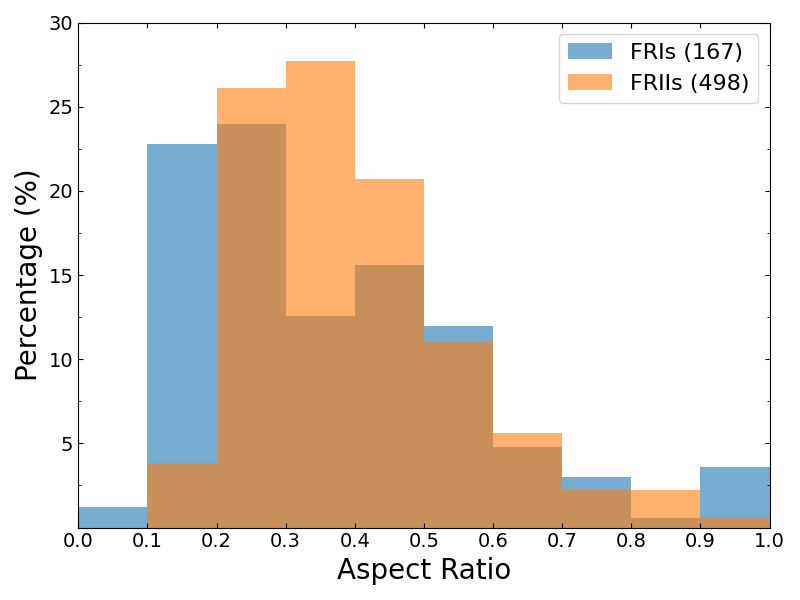
\includegraphics[width=0.9\linewidth]{Figure/Section 4/AxisRatio.png}
    \caption{Based on the elliptical structures illustrated in \autoref{fig:Figure2}, the axis-ratio distributions for FRIs and FRIIs can be statistically derived.}
    \label{fig:AxisRatio}
\end{figure}
\begin{figure*}[!htbp]
    \centering
    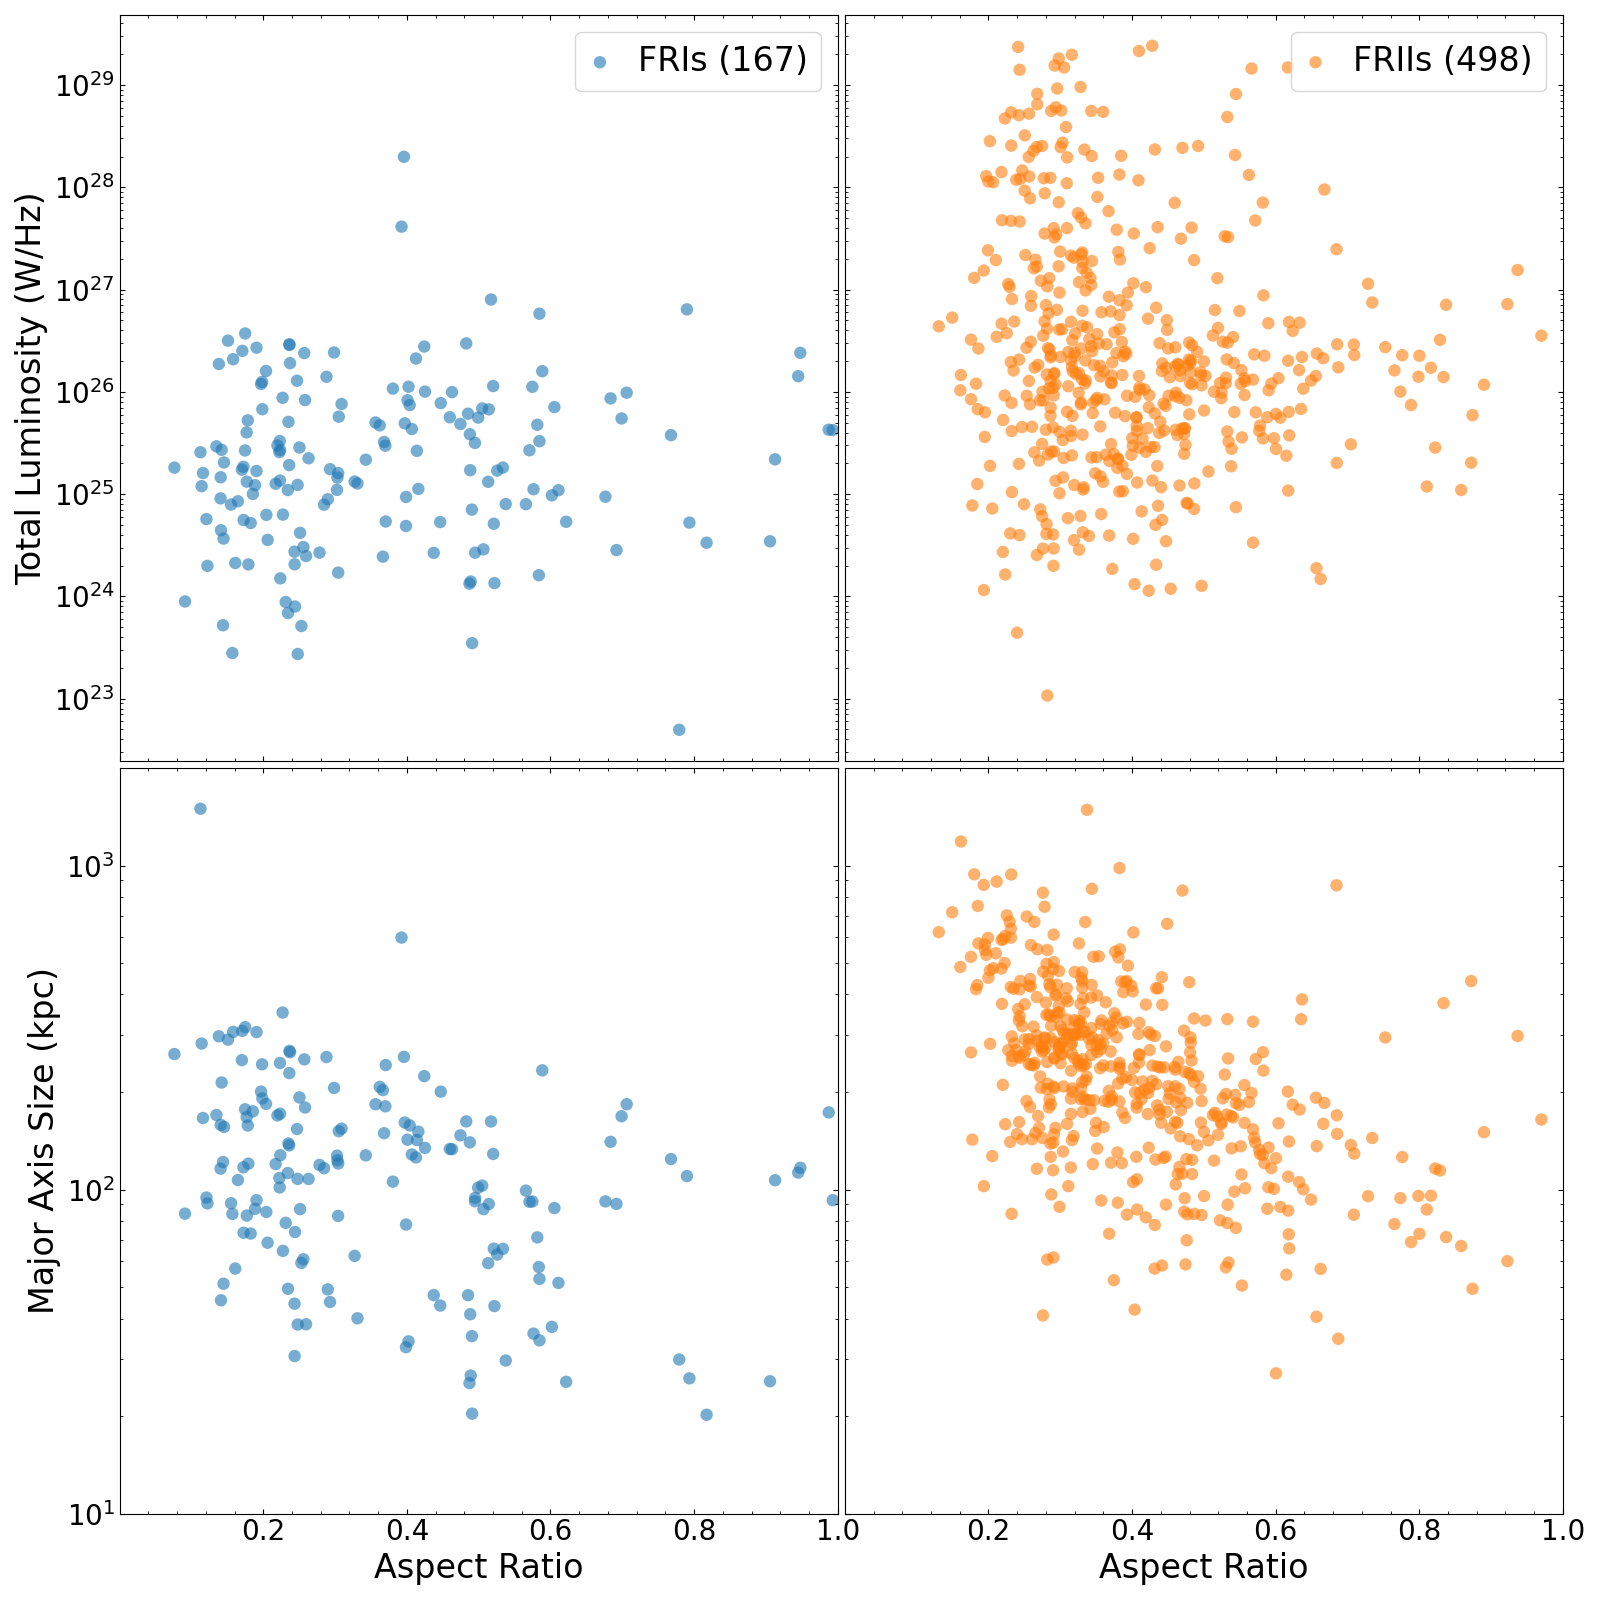
\includegraphics[width=0.8\linewidth]{Figure/Section 4/AxisRatioRelationship.png}
    \caption{Presented here are the underlying distribution characteristics of the aspect ratio relative to total luminosity and elliptical major axis size for RGs of different FR types. A distinctly offset distribution is clearly observed between the FRI-type and FRII-type populations in the figure.}
    \label{fig:AxisRatioRelationship}
\end{figure*}
\begin{figure}[!htbp]
    \centering
    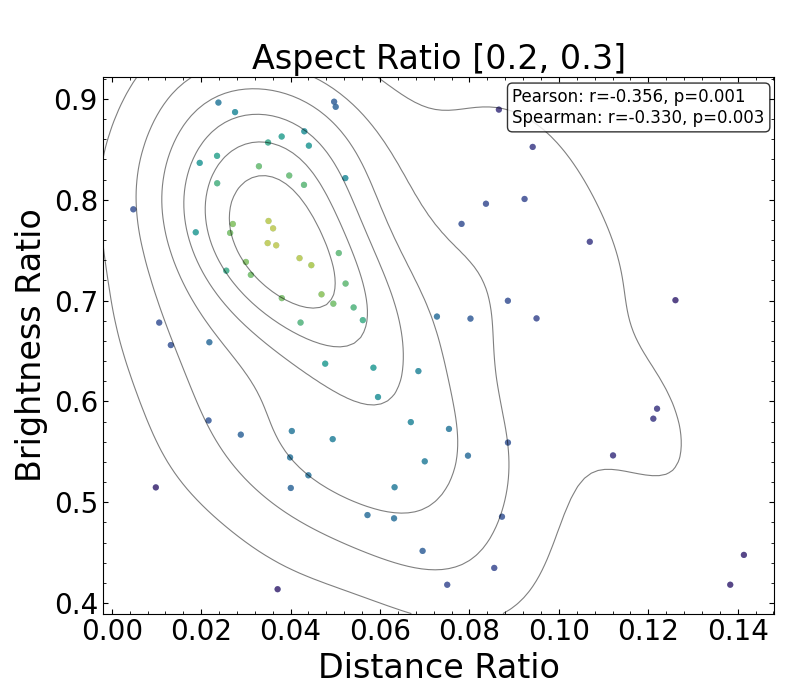
\includegraphics[width=0.8\linewidth]{Figure/Section 4/DistanceBrightnessRelationship.png}
    \caption{This figure illustrates the potential correlation between the separation of the double lobes and the brightness distribution for FRIIs within a specific range of aspect ratios. The horizontal axis represents the ratio of the double-lobe distance to the elliptical major axis size of FRIIs, while the vertical axis denotes the ratio of the radio brightness on the two sides, obtained by dividing each FRII into two parts centered on its optical counterpart. The brightness contribution from any radio lump coinciding with the optical counterpart is excluded from the calculation.}
    \label{fig:DistanceBrightnessRelationship}
\end{figure}

\begin{figure*}[!htbp]
    \centering
    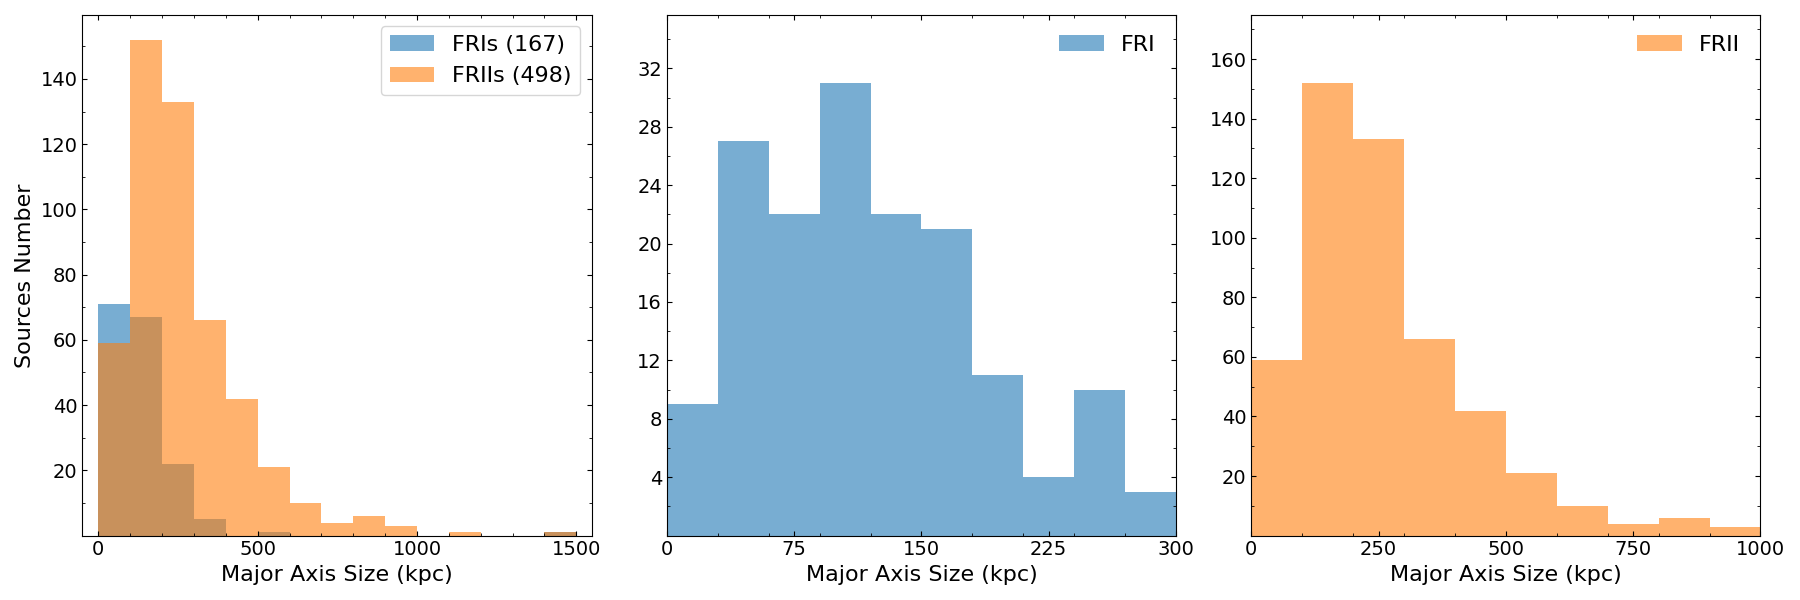
\includegraphics[width=0.9\linewidth]{Figure/Section 4/Max_Scale_Distribution.png}
    \caption{Based on the major axes of the ellipses illustrated in \autoref{fig:Figure2}, the elliptical major axis size distributions for FRIs (left panel) and FRIIs (right panel)  can be statistically derived.}
    \label{fig:Max_Scale_Distribution}
\end{figure*}




\subsection{The Statistical Characteristics of $r_s$}\label{sec:Section4_3}

% 介绍r_s
In order to compare with previous results and validate our results, we first show the $r_s$ function in \autoref{fig:r_s_distribution0} for FRIIs. 
It can be seen that our results agree with \citet{lin_populations_2010}, both showing two significant peaks around 0.15 and 0.60. 
Although this results show a gap between 0.2 and 0.4 and minor peaks near 0.5 and 0.8, the overall discrepancy is acceptable. On the one hand, some sources were excluded from our sample. On the other hand, we employ a uniform method to determine the $r_s$ for all sources, whereas \citet{lin_populations_2010} applied different approaches for different source types.
% \textbf{Here the sources with $r_s<0.3$ should be not identified with $r_s$ \citep{}. These sources shows close radio knots and weak emission extending long distances.}


Compared with \citet{lin_populations_2010}, the FRIIs in this work display more distinct and isolated features in the regime of $r_s < 0.3$. 
Physically, $r_s < 0.3$ corresponds to a configuration where the separation between the two hotspots is significantly smaller relative to the total extent of the radio structure. This characteristic primarily arises from prominent outflow-like structures: hotspot-centered clumps extend outward in multiple directions. When such extended emission is not aligned with the optical counterpart (or central clump), the fitting algorithm expands the ellipse to satisfy the required coverage fraction, ultimately yielding a hotspot separation that is notably small relative to the ellipse major axis. 
Based on this methodology, a distinct structural subclass can be identified within this $r_s < 0.3$ range.


However, is an excessively stringent coverage rate the dominant factor influencing the fitting of elliptical Gaussian components for hotspots? 
In the procedure illustrated in \autoref{fig:Different_rs}, the coverage rate of elliptical Gaussian components is gradually reduced (set to 95\%, 90\%, 80\%, 70\%, 60\%, and 50\%, respectively), with both peak positions and the overall distribution remaining stable. As coverage constraints are relaxed, faint outflows on both sides of the lobes are the first to be excluded from the fitted ellipses; nevertheless, these features exert no significant influence on the stability of the subclass structures.
This confirms the robustness of the substructure within the $r_s < 0.3$ range.


\begin{figure*}[!htbp]
    \centering
    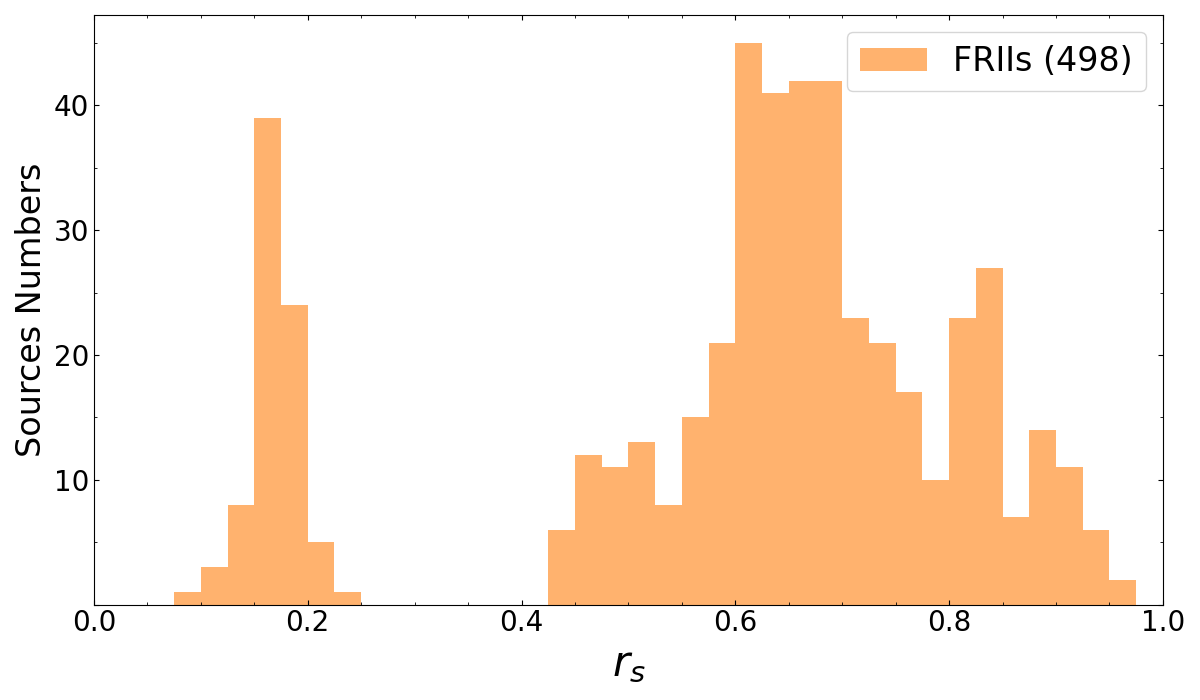
\includegraphics[width=0.45\linewidth]{Figure/Section 4/r_s_distribution0.png}
    \caption{
    Presents the distribution of $r_s$ for brightness thresholds of 95\% (blue) and 50\% (blue, completely obscured by the underlying wine red).
    }
    \label{fig:r_s_distribution0}
\end{figure*}


% Nodes分布特征
\subsection{The Node Structure of RGs}\label{sec:Section4_4}

% 介绍knots
During processing in \autoref{sec:Section3_3}, interest in knot structures emerged, leading to the incidental development of a counting method. This method is straightforward: building on the aforementioned flood-filling approach, a threshold (as a percentage of the central clump's maximum brightness, here is 0.5\% by step) is incrementally increased to constrain the RG extent. Distinct knots are revealed in this process\textemdash with rising thresholds, knots originally blended in lobes gradually separate, then fade, leaving only the bright core (similar to \autoref{fig:KnotSimple}). A key distinction must be clarified before presenting results: "knot" refers to clumpy structures excluding the bright core in FRIs, whereas "node" includes the bright core.
Knots are larger than one pixel and remain exist when the increment of the threshold is higher than 2 percent, which are not likely to be due to fluctuation, and should be the radio knots.

% 介绍曲线
The total number of knots in FRIs and FRIIs is investigated as presented in \autoref{fig:Node_Evolution}. For a given brightness threshold, the number of nodes identified across all RGs is summed to derive the variation in total node count as a curve of the adopted threshold.
As the threshold increases to 15\%, knot structures emerge in an increasing fraction of sources, followed by a gradual deceleration in this trend. A transitional feature appears at the 75\% threshold, beyond which the overall trend becomes markedly pronounced.

% 曲线的区别
Notably, distinct morphological differences are present between FRIs and FRIIs (it explain reason why bias between two curves), characterised herein by the node count ($count_n$) and knot count ($count_k$). Morphologically, FRIs always host a bright central core($count_n \geq 1$ and $count_k = count_n -1 $). By contrast, FRIIs may display only two bright lobes ($count_n \geq 2$ and $count_k = count_n -2 $), or harbour an additional bright central core ($count_n \geq 3$ and $count_k = count_n -3 $); As the threshold increases in the subsequent process, the node count of FRIIs declines progressively, ultimately leaving either one core plus one lobe ($count_k = count_n -2 $) or a single core or lobe ($count_k = count_n -1 $).
% 具体的区别
Notably, the orange curve exhibits an initial downward followed by a persistent upturn trend, a feature absent in the blue curve; this discrepancy arises because low-flux faint cores and lobes dissipate rapidly at early stages. Within the threshold range of 15\% to 75\%: the blue curve displays a fluctuating declining trend, governed by the inherent instability of knot structures, because individual knots split into numerous small sub-nodes and gradually fade out as the threshold increases; in contrast, the orange curve maintains a steady, smooth downward trend, as a large population of stable persistent nodes (associated with lobes or cores) mitigates the structural instability of knots. For thresholds exceeding 75\%, both the blue and orange curves undergo a pronounced accelerated decline, owing to the fact that all RGs ultimately evolve into compact pure nuclear clumps.


\begin{figure*}[!htbp]
    \centering
    
\includegraphics[width=0.3\linewidth]{Figure/Section 4/KnotSimple1.png}
    
\includegraphics[width=0.3\linewidth]{Figure/Section 4/KnotSimple2.png}
    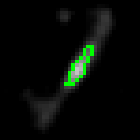
\includegraphics[width=0.3\linewidth]{Figure/Section 4/KnotSimple3.png}
    \caption{By applying the flood-filling algorithm, knots within RGs are gradually revealed and subsequently disappear as the threshold increases.}
    \label{fig:KnotSimple}
\end{figure*}

\begin{figure*}[!htbp]
    \centering
    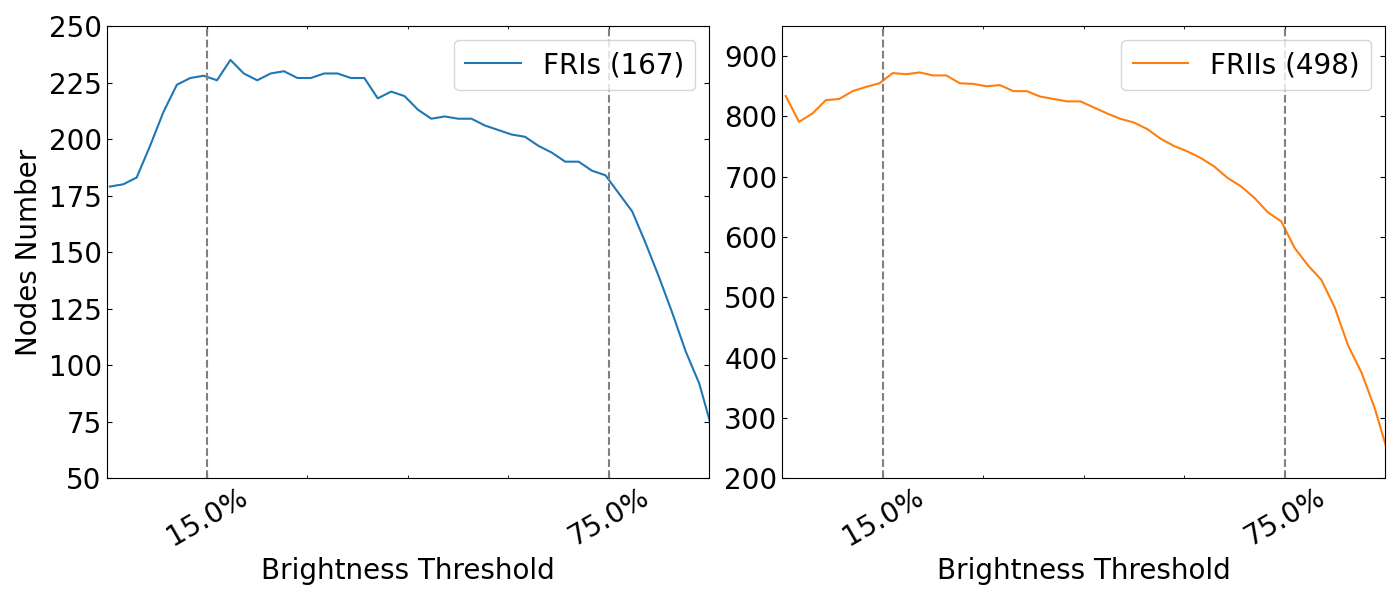
\includegraphics[width=0.9\linewidth]{Figure/Section 4/Node_Evolution.png}
    \caption{Based on the flood-filling algorithm illustrated in \autoref{fig:KnotSimple}, the total number of knots in the sample can be quantified and presented. To reduce the influence of statistical fluctuations, a threshold interval of 2\% peak brightness is adopted for the abscissa in the figure. In practice, the algorithm uses a step size of 0.5\% of the peak brightness, which may be overly fine for some faint sources. }\label{fig:Node_Evolution}
\end{figure*}
% \clearpage



\subsection{The Feature of Central line Brightness Stacking Curve}\label{sec:Section4_5}

In addition to the overall radio morphology, the intensity distribution provides more detailed information about the RGs. 
Here we use a curve referred as central line to describe the direction of the jet flow, and adopt the intensity along the line as the representative of the intensity distribution.
However, for FRIs, radio emission extends across a broad range, rendering the central line ineffective for analysis. Accordingly, investigations of the central line are confined solely to FRIIs.
The left panel of \autoref{fig:CentralLine} shows a example of the identified central lines for the RG. It can be seen that the central lines are feasible to mark the trajectories of the radio structure centers.


To assess the error budget, three factors are considered in this work. First, the FIRST official website specifies a typical rms of 0.15 mJy, while rms values derived from cropped images deviate from this reference. Second, VizieR notes that for bright sources, the accuracy of Fpeak is limited to approximately 5\% due to systematic effects. Third, a code modification for pixel position bias correction is introduced, which simulates pixel position deviations in the calculation of the horizontal axis physical scale to estimate errors caused by pixel discretization. However, minor deviations from redshift and cosmological models are not considered. Additionally, the error propagation formula is applied to each calculation step. Finally, red shaded regions are used to represent the errors in \autoref{fig:FR_StackingCurve}.
Additional analysis is conducted on the radio emission along the central line to establish a general overview of the overall structural characteristics. For the calculation of 1.4 GHz radio luminosity, the formula cited in \cite{koziel-wierzbowska_2021} is adopted, with $\alpha$ set to 0.75 as the mean spectral index for sources detected at 1.4 GHz.

% 光度范围过大，可以归结为“选取的中心线往往是RG最亮的位置”，所以换算得到的光度就比一般的RG更亮得多
Notably, as shown in \autoref{fig:FR_StackingCurve}, the stacking curve ranges from $ 10^{31}\ W\ \text{Hz}^{-1}\ \text{kpc}^{-2} $ to $ 10^{33}\ W\ \text{Hz}^{-1}\ \text{kpc}^{-2} $. Given that the order of magnitude of the number of stacked RGs is approximately $ 10^{3} $, and the selected regions correspond to the brightest "central line" regions across the entire RGs, the derived luminosity exceeds the typical luminosity range of FRII galaxies, which is between $ 10^{25}\ W\ \text{Hz}^{-1}  $ to $ 10^{29}\ W\ \text{Hz}^{-1} $\citep[e.g.,][]{an_dynamic_2012}.
% 为什么堆叠曲线的FRIIs与前面统计的506数量不同？


\cite{turner_energetics_2015} previously proposed an evolutionary model for FRI/FRII radio AGNs and their mutual transitions. To reveal the dynamical mechanisms of jet-ambient medium interactions, they developed a comprehensive model that encompasses the supersonic, transonic, and subsonic phases of jet-cocoon expansion, alongside a comparative pure FRII model (where jets maintain supersonic expansion throughout their entire lifecycle). Thus, how can these characteristics be captured?
Here, the use of the central line to characterize the brightness distribution of RG is proposed. Constrained by observational resolution, only the most prominent regions can be focused on; nevertheless, stacking these prominent regions may uncover characteristics of the population evolution of FRIIs.


The central lines of FRIIs are split at their optical counterparts \textemdash thereby doubling the sample size \textemdash and the brightness distributions of all sample central lines are stacked, from which the brightness stacking curve presented in \autoref{fig:FR_StackingCurve} is derived. The statistically derived brightness-stacked profiles of FRIIs exhibit structural similarity to their luminosity-size profiles: the brightness stacking of FRIIs features multiple peak regions, indicating the presence of multiple radiation-active regions; beyond 100 kpc from the optical counterpart, a steep decline follows where brightness decreases rapidly with increasing distance.
Notably, the FRI population does not exhibit significant characteristics and is therefore not presented herein.


\begin{figure}[!htbp]
    \centering
    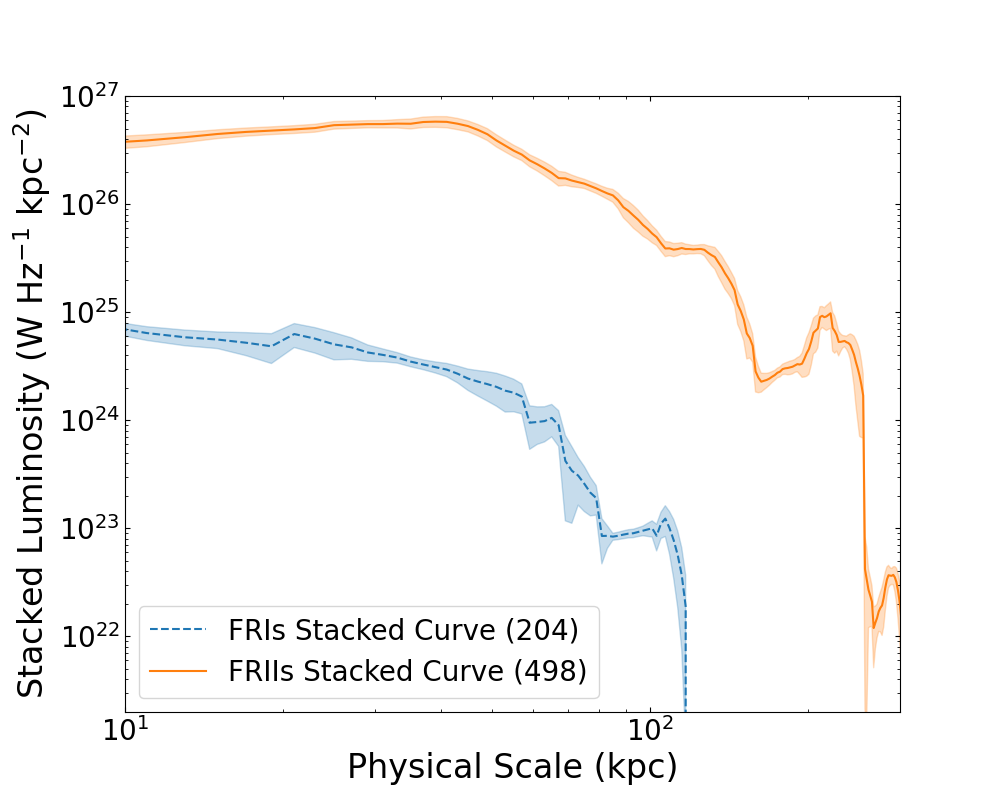
\includegraphics[width=0.9\linewidth]{Figure/Section 4/StackingCurve.png}
    \caption{Based on the flood-filling algorithm illustrated in \autoref{fig:CentralLine}, the central-line brightness stacking curve for FRIIs is presented here. In contrast to the display in the right panel of \autoref{fig:CentralLine}, each single central line of an RG is folded about its center to yield two brightness profiles, which are subsequently stacked together. This figure presents the final stacked average brightness profiles derived from 206 FRIs (blue curve) and 375 FRIIs (red curve), respectively, where the shaded region denotes the uncertainty in the brightness distribution. }
    \label{fig:FR_StackingCurve}
\end{figure}


    % 由于之前提到不再讨论倾角问题，所以伸长参数这一块还是不写了
        % % 伸长参数
        % \subsection{The Distribution of Elongation Parameter}\label{sec:Section4_6}
        
        
        % \begin{figure*}
        %     \centering
        %     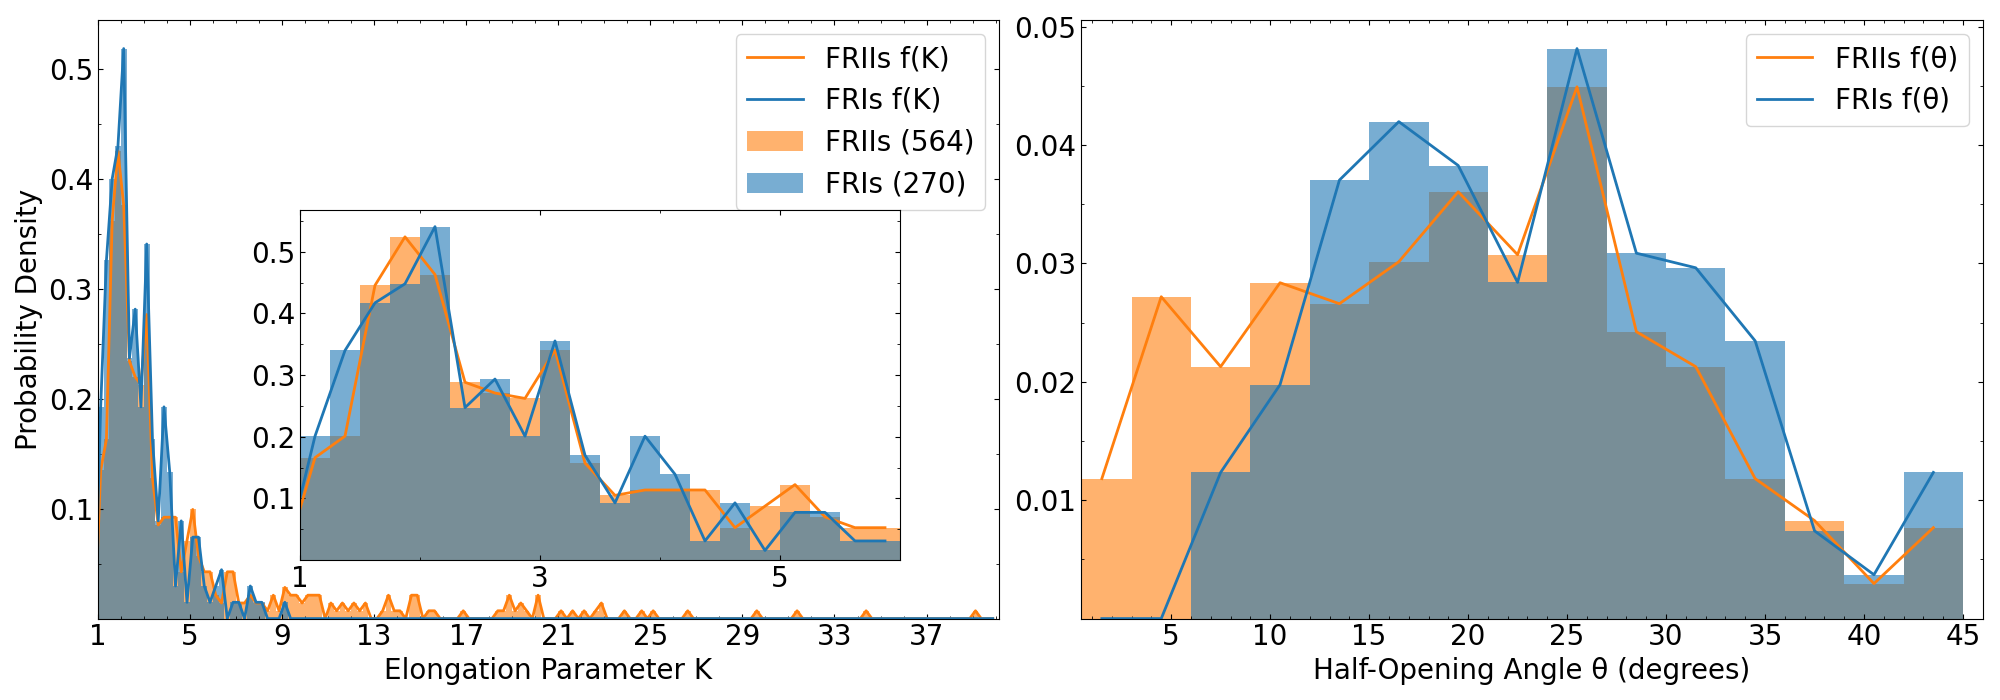
\includegraphics[width=0.9\linewidth]{Figure/Section 4/ProbabilityDensity.png}
        %     \caption{Left Panel: Probability density distribution of the elongation parameter K; The horizontal axis represents K, and the vertical axis denotes the probability density of K; Histogram bins for K are set at intervals of 0.25, with the corresponding curve $f(K)$ representing the probability density function of K; Red and blue colors correspond to FRIs   本公司 and    和FRIIs, respectively. Right Panel: Probability density distribution of the half-opening angles ($\theta$) of RGs   该公司 estimated using K; The horizontal axis represents the $\theta$, and the vertical axis denotes the probability density of the $\theta$; Histogram bins for the $\theta$ are set at intervals of $3^\circ$ , with the corresponding curve $f(\theta)$ representing the probability density function of the $\theta$.}
        %     \label{fig:14}
        % \end{figure*}
        % % \clearpage


\section{Discussion}\label{sec:Discussion}

\subsection{The Deviations in Procedure}\label{sec:Section5_1}
% 大概介绍一下对源处理的偏差
% 1.光学对应体匹配
In practice, genuine optical counterparts may remain unmatched due to observational limitations. Consequently, a substantial fraction of RGs lacking matched optical counterparts must be excluded from our program. The matching status of optical counterparts is illustrated in \autoref{fig:OpticalCounterpartCountDistributions}.

    % 由于之前提到不再讨论倾角问题，所以argue一下星系倾角问题这一块还是不写了
    % % 2.argue一下星系倾角问题！从各向同性出发，参考其他人的文章。
    % In observational studies of radio galaxies, the inclination angle problem has long been a core challenge plaguing astronomers. The inclination angle is defined as the angle between the axis of symmetry of a radio galaxy and the observer’s line of sight, and this seemingly straightforward geometric parameter actually encapsulates highly complex physical information. Since the observed radio galaxy images are essentially the projection of three-dimensional structures onto the two-dimensional celestial sphere, different inclination angles can result in entirely distinct observed morphologies for the same intrinsic structure \citep{reynolds_projection_1980}. The degeneracy arising from this projection effect renders the extraction of true physical parameters from observational data extremely challenging. With the continuous advancement of technology, several methods based on isotropy to infer the inclination angle have emerged \citep[e.g.,][]{schmitt_jet_2001,drouart_jet_2012,oei_discovery_2022}, but these approaches impose non-trivial requirements on observational data and telescope resolution\textemdash requirements that are not easily satisfied in the work presented in this paper.

% 3.高斯椭圆的结构其实也有问题
Additionally, Gaussian elliptical fitting for component extraction requires attention. With fewer constraints, its fitting accuracy may decrease, necessitating extensive manual inspection to identify poor fits and ensure high-quality source extraction. Thus, complex Gaussian fitting is unsuitable for large-scale survey data analysis; it may even cause catastrophic errors when applied to highly distinct RGs. However, it remains adequate for component extraction in simple scenarios. Notably, when constraining component division for RGs, we adopted a strict 95\% brightness threshold for FRIIs but only 80\% for FRIs. This is due to the general characteristics of FR types: FRIs often have faint, diffuse edge structures that severely hinder key region identification, whereas the more regular structure of FRIIs allows for stricter constraints. There may be cases of failure to match an ellipse.

% 4.中心线定位并不准确
In this study, the BSF is utilized to locate the central line; however, this method may introduce deviations. Specifically, this localization process is analogous to pruning, which tends to eliminate "extraneous branches" in regions with complex structures. Naturally, the structural features exhibited in complex regions undergo a more pronounced simplification than those in simple regions. Nevertheless, the present method offers distinct advantages over conventional ridge-line-based techniques. Specifically, the quality of ridge lines is highly dependent on image preprocessing steps, and they are less suitable for RG systems featuring large gaps or curved head-tail structures \citep[e.g.,][]{barkus_application_2021,clews_radio-loud_2025}.



\begin{figure}
    \centering   
    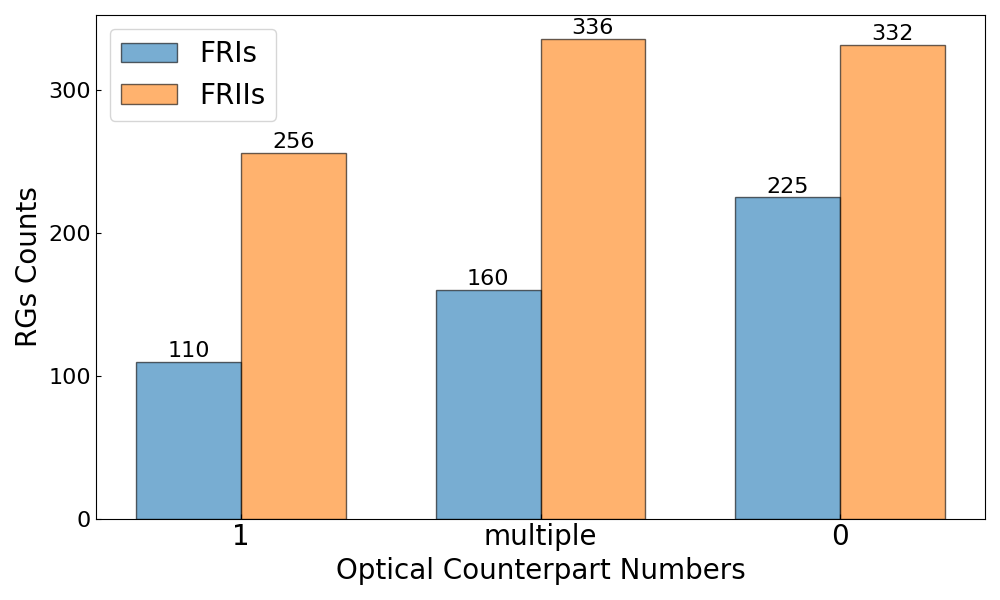
\includegraphics[width=0.9\linewidth]{Figure/Section 5/OpticalCounterpartCountDistributions.png}
    \caption{This figure illustrates the distribution of RGs during the search for their optical counterparts. The two colored labels correspond to FRI/FRII-type RGs, respectively. The horizontal axis represents the number of optical counterparts detected for each RG: optical counterparts with a detection count of 1 are relatively more reliable than those with a count of "multiple", and RGs with an optical counterpart count of 0 will be excluded from our subsequent analysis. The vertical axis denotes the number of RGs.}
    \label{fig:OpticalCounterpartCountDistributions}
\end{figure}



\subsection{The Relation between Aspect Ratio, Scale, Brightness}\label{sec:Section5_2}

% 在特定轴比下的double lobe的 尺度比-亮度比 相关性
Is there a correlation associated with aspect ratio, scale, and brightness simultaneously? 
In such a simple elliptical model, there is no definitive empirical relationship; however, the positional deviation between the optical counterpart and the radio source, as well as the existence of the Doppler effect, are objective facts. 
The former can be represented by the distance ratio, which is calculated as the distance between the geometric center of the ellipse and the optical counterpart divided by the major axis of the ellipse. The latter can be characterized by a brightness ratio, defined as the ratio of the brightness of the darker side to that of the brighter side when the RG is bisected into two equal halves by a straight line passing through the optical counterpart and perpendicular to the major axis. Subsequently, RGs are divided into 10 sample groups with an equal interval of 0.1 in aspect ratio.
Based on the above assumptions, we aim to find samples with small positional deviations of the optical counterpart and non-extreme Doppler effect, and observe their distribution. Surprisingly, in the distance ratio - brightness ratio plane under specific aspect ratios (see \autoref{fig:DistanceBrightnessRelationship}), the sample distribution unexpectedly exhibits a certain degree of correlation.

% 解释
This inference can be drawn under a physical scenario: for RGs with weak external perturbations, large-scale double radio lobes form first. Due to the inclination between the global structure and the line of sight, the lobe oriented toward observers appears extended and luminous, whereas the counter lobe is compact and faint. This projection effect ultimately produces positional offsets of the optical counterparts in the observed plane.
In line with this interpretation, \autoref{fig:DistanceBrightnessRelationship} shows that a stronger brightness asymmetry between the two lobes (a smaller brightness ratio) correlates with a larger positional deviation of the optical counterpart (a larger distance ratio). Such a correlation is only evident for RGs with an aspect ratio in the range of [0.2, 0.3], which may reflect that RGs within this range possess stable intrinsic structures and experience minimal environmental disturbance.


%  椭圆轴比聚集于0.3，FRIs比FRIIs更弥散——相似的演化机制？
Although the sample size of FRIs is smaller than that of FRIIs, the overall axial ratio distribution of FRIs is considerably more dispersed in \autoref{fig:AxisRatio}. Given that FRIIs typically host more powerful central engines than FRIs, their jets may be less susceptible to environmental effects. Here, a distinct clustering in the FRII distribution is evident, suggesting that FRII radio lobe structures naturally tend toward axial ratios approaching 0.3. Notably, the peak of the FRI distribution also lies near an axial ratio of 0.3. In \autoref{fig:AxisRatio}, the discrepancy in physical scale distributions between FRIs and FRIIs is clearly observable and remarkably large; nevertheless, both the axial ratio and elongation parameter exhibit similar distribution patterns across the two classes. This observation implies the existence of a shared mechanism of morphological evolution in FR-type RGs. 
From the evolutionary pathways presented in \cite{An and Baan, 2012}, the evolution of FRIIs transitioning from compact symmetric objects to large-scale symmetric objects reveals that these sources may naturally evolve into FRIs upon reaching the regime of jet instability.

\begin{figure}[!htbp]
    \centering
    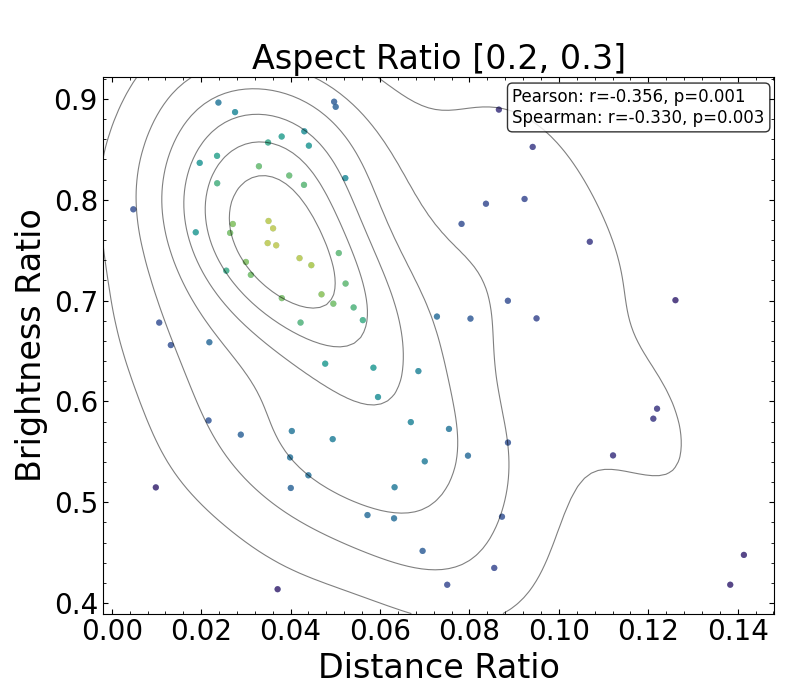
\includegraphics[width=0.8\linewidth]{Figure/Section 4/DistanceBrightnessRelationship.png}
    \caption{This figure illustrates the potential correlation between the separation of the double lobes and the brightness distribution for FRIIs within a specific range of aspect ratios. The horizontal axis represents the ratio of the double-lobe distance to the maximum scale of FRIIs, while the vertical axis denotes the ratio of the radio brightness on the two sides, obtained by dividing each FRII into two parts centered on its optical counterpart. The brightness contribution from any radio lump coinciding with the optical counterpart is excluded from the calculation.}
    \label{fig:DistanceBrightnessRelationship}
\end{figure}



\subsection{The Mechanism of Knot}\label{sec:Section5_3}

\cite{mizuno_recollimation_2015} investigated the physical mechanism of jet recollimation and conducted relevant numerical simulations. Their findings indicated that AGN jets narrow and brighten at a characteristic length scale while interacting with the ambient cosmic environment. Furthermore, knots observed in NGC 2663 offer evidence for recollimation in FRIs \citep{velovic_collimation_2022}. In contrast, the present study puts forward a critical doubt: could the variations in node number reported in this research be attributed to sporadic brightness fluctuations?

% 讨论Node的变化是否合理——排除涨落的特征
By nature, random fluctuations are characterized as unpredictable small-amplitude variations, corresponding to a significantly low Coefficient of Variation (CV). In contrast, structural changes manifest as systematic variations with inherent regularity, where the CV assumes a moderate value and is accompanied by distinct trend-like features. 
Thus, the CV can be employed as a quantitative metric to discriminate between fluctuations-driven and structure-driven variations. For non-negative normally distributed variables, the sample $\mathrm{CV}$ is defined as the ratio of the sample standard deviation to the sample mean: $\mathrm{CV} = \frac{\sqrt{S^2}}{\bar{x}},$ where $S^2$ denotes the sample variance and $\bar{x}$ represents the sample average.


% 对于FRIs
In the FRI sample, 120 sources ($\approx 71.0\%$) possess a brightness variation coefficient of $CV \geq 0.05$, with a mean nodal count of 1.356 measured for this subset. Additionally, 104 FRI-type sources ($\approx 61.5\%$) host persistent knots extending across continuous brightness intervals exceeding 2\%. Only a small fraction of FRIs contribute no measurable knot counts, whereas the majority of the sample exhibits prominent variability signatures that reveal statistically significant variations in knot properties.

% 对于FRIIs
In contrast, quantitative characterisation of FRIIs remains challenging due to their highly complex and diverse structural morphologies. Among the FRII population, 500 sources ($\approx 98.8\%$) show $CV \geq 0.05$ in brightness variation, corresponding to a mean nodal count of 1.597; and 497 FRIIs ($\approx 98.2\%$) feature persistent knots within continuous brightness intervals greater than 2\%. It should be noted that the statistical analysis of FRIIs' knots is likely affected by considerable systematic bias: the nodal structures of FRIIs are heterogeneous and cannot be easily disentangled to enable clear knot segregation and counting. Even so, the overall statistical trend confirms that the variability amplitude of knots in FRIIs is distinctly higher than that in FRIs.

% 综上所述，FRI/FRII 不同的knot是否说明它们当前的演化区别？
\cite{an_dynamic_2012} discussed that during FRII evolution, high-power laminar-flow jets \textemdash although largely invisible \textemdash form a stagnation point within the radio lobe. As the jet boundary layer dissipates kinetic energy through viscous entrainment and fluid instabilities, and these processes extend toward the jet central line, the jet loses much of its energy and momentum, eventually becoming diffuse and poorly defined, as observed in FRIs.
Within this physical framework, knots in FRIIs are expected to occur far more frequently and show significantly more pronounced variations than in FRIs, a behavior that is also reflected in the CV presented in this paper.
% knots数量似乎跟recollimation无关
Furthermore, within the present dataset, it is evident that not all sources follow the characteristic whereby a greater number of knots corresponds to enhanced collimation of RG lobes. Further visual examination of the sample reveals no definitive correlation between knot abundance and enhanced collimation of RG structures.



\subsection{Orientation Effect} \label{subsec:Section5_4}
As shown in \autoref{fig:Redshift&MassDistribution}, the FRI and FRII subsamples exhibit broadly similar black hole mass distributions, whereas the galaxy stellar mass distribution of the FRII is systematically shifted toward lower values relative to that of the FRI population. The observed difference between the two populations is therefore unlikely to be explained solely by a systematic difference in black hole mass. 

Radio-mode AGN feedback provides one possible physical connection between radio activity and host galaxy evolution. 
In this scenario, the accretion produces mechanical energy in the form of radio jets. 
In galaxies with quasi-hydrostatic hot halos, this energy can offset radiative cooling and reduce the supply of cold gas available for star formation \cite{Somerville & Davé - 2015, Bower et al. 2006}. 
The resulting suppression of gas condensation and star formation limits subsequent galaxy stellar mass growth and helps prevent the formation of excessively massive galaxies \cite{Croton et al. 2006, Lagos et al. 2008}. This process may be summarized as
\[
P_{\rm jet}\uparrow
\;\longrightarrow\;
\dot{M}_{\rm cool}\downarrow
\;\longrightarrow\;
{\rm SFR}\downarrow
\;\longrightarrow\;
\frac{{\rm d}M_\star}{{\rm d}t}\downarrow .
\]

Repeated or long-lived feedback episodes can reduce the amount of galaxy stellar mass subsequently formed. Classical semi-analytic implementations represent this process phenomenologically by suppressing gas cooling rather than by explicitly resolving the propagation and thermalisation of radio jets \cite{Croton et al. 2006}. Observationally, large scale FRII radio lobes have also been associated with stronger suppression of star formation in surrounding satellite galaxies than compact radio sources, supporting the idea that extended radio structures trace physically significant kinetic feedback \cite{Wang et al. 2026}. 

More importantly, although jet orientation can alter the projected size and appearance of a radio source, it would not naturally produce a systematic offset in a host property such as galaxy stellar mass. If FRIs and FRIIs were intrinsically similar systems whose morphological differences arose solely from viewing angle or projection, their galaxy stellar mass distributions would be expected to be broadly comparable. Instead, our FRIIs show both more prominent extended radio activity and a galaxy stellar mass distribution centred at a lower value than that of the FRI hosts, despite the similarity of their black hole mass distributions. This combination suggests that the FRI/FRII separation in our sample is primarily associated with intrinsic differences between the two populations rather than being solely an orientation induced effect. 


\section{Conclusions and Future} \label{sec:Conclusions and Future}

\subsection{Conclusions}\label{sec:Conclusions}

The objective of this work is to integrate existing research methodologies to conduct a deeper geometric analysis of RG structures based on FR-classified 1.4 GHz images.
The prevailing perspective on jets and radio lobes predominantly attributes their physics to shock-initiated processes. Within this consensus, we propose that elliptical geometries can effectively characterize FR-classified RGs. To derive optimally constrained elliptical structures, we employed Flood-filling algorithms, optical counterpart matching, and central line construction, ultimately generating tailored elliptical models for FRI and FRII morphologies. Crucially, our methodology aims to develop a universal framework adaptable to diverse RG shapes, not limited to ellipsoidal forms. 

Consequently, we identified four distinct descriptive perspectives for RGs in the discussion section. Our analysis can be summarised as follows:

\begin{itemize}[label=$\star$]

    % axis ratio
    \item We performed a statistical analysis of the morphological properties of RGs and constructed scatter plots for central black hole mass, stellar mass, total luminosity, maximum physical scale, aspect ratio, and central line integral ratio. We focus on characterising the statistical structural signatures of RGs using the aspect ratio, and establish its correlation with total luminosity and maximum source scale. Beyond refining the existing understanding of FR morphological classification, this study further quantitatively verifies the physical differences between FRI and FRII populations. 
    Additionally, within the restricted aspect ratio range of [0.2,0.3], a clear correlation emerges between the double-lobe brightness ratio and the positional offset ratio of their optical counterparts.

    % r_s
    \item Subsequently, we adopted the classical $r_s$ method for sample analysis and compared our findings with the results presented in \citet{lin_populations_2010}. A distinct substructure was identified for FRIIs in the regime $r_s$ < 0.3, with most such features corresponding to outflow-like structures. This substructure proves insensitive to algorithm parameter adjustments and can persist stably across different tuning configurations.

    % knot
    \item The second perspective focuses on knot enumeration for FRI sources. A flood-filling approach with a maximum brightness threshold was adopted to track the evolutionary characteristics of knot structures. We analysed the variation trends of knot counts, and CV validation confirmed that these knots are not induced by random flux fluctuations.
    
    \item Finally, brightness stacked profiles. By leveraging the requirement to locate optical counterparts, we derived a curve describing both geometric and brightness characteristics of RGs—namely, the center line. Subsequently, stacking the brightness distributions of center lines from a sufficient sample size naturally reveals the average radiatively active regions.
    
\end{itemize}

Integrating these perspectives collectively, this work provides improved clarity on the structural properties and evolutionary mechanisms of FR-classified RGs.




\subsection{Future}\label{sec:Future}

% 基本意义
The original objective of this project is to extract statistical parameters that can characterize the structure of RGs from the sample distributed at 1.4 GHz. 
The Murchison Widefield Array has obtained deep EoR images toward specific sky fields \citep{offringa_parametrizing_2016} and revealed dense extragalactic sources. These sources act as both the observational background for the 21 cm forest and potential foreground contaminants.
Some methods of foreground source modeling need subtract bright sources at the first \citep{di_matteo_radio_2002,di_matteo_21-cm_2004}.  
A qualitative understanding of the structure of foreground sources is required; for example, Independent Component Analysis of \cite{chapman_foreground_2012} relies on observational constraints and physical models derived from RGs. The simple method and derived parameters presented in this paper allow for a fundamental characterization of their structure.

% 提及应用前景
This work is anticipated to undergo further development and support simulation efforts in future research, including modeling jet structures for different RGs to refine the authentic jet-lobe morphologies observed by various telescopes. Furthermore, radio lobe structures may exhibit relevant interactions with the interstellar medium or intracluster medium; the description of these structures can be used to characterize the interactions between jets and the medium, and also reflect the kinematic components of the intergalactic medium as well as the characteristics of host galaxies. Additionally, special types of RGs will also be key research directions in the future, such as Giant RGs and Hybrid Morphology RGs.
Additionally, the fine sub-kiloparsec scale structures of radio-quiet AGNs \citep[e.g., those detected in J0802+4643][]{vardoulaki_fr-type_2021} can fill the statistical gaps in this work, and the development of future radio telescopes will further expand the understanding of RG structures.




\bibliographystyle{aa}
\bibliography{BibDir/Introduction,BibDir/Data,BibDir/Method,BibDir/Discussion}
\begin{appendix}
\section{Alternative thread identification}\label{app:Alt} 




\end{appendix}






\end{document}

